% !TEX TS-program = xelatex
% !TEX encoding = UTF-8 Unicode

\documentclass[a4paper, 12pt]{report}

\usepackage[utf8]{inputenc}
\usepackage[T1]{fontenc}

\usepackage[]{geometry}
\usepackage[english]{babel}
\usepackage{graphicx}
\usepackage[hidelinks]{hyperref}
\usepackage{multirow}
\usepackage{float}
\usepackage{url}
\usepackage{hyperref}
% \usepackage{xcolor}

% Color table cells
\usepackage[table]{xcolor}

% For subscript? 
\usepackage{fixltx2e}
\usepackage{hyperref}

% Page numbering - roman
\pagenumbering{roman} 

% Add references to TOC
\usepackage[nottoc,notlof,notlot]{tocbibind} 

% Rename Bibilography to References
\addto\captionsenglish{\renewcommand{\bibname}{References}}

% Change section numbering to start from 1.0
% \renewcommand*\thesection{\arabic{section}.0}
% \renewcommand*\thesubsection{\arabic{section}.\arabic{subsection}}

% Font
\usepackage{fontspec}
\defaultfontfeatures{Mapping=tex-text,Scale=MatchLowercase}
\setmainfont{Times}

% Font size
\usepackage{titlesec}
\usepackage{sectsty}
\sectionfont{\fontsize{16}{18}\selectfont}
\subsectionfont{\fontsize{14}{16}\selectfont}

% Set emergency stretch - Avoid overfull \hbox
\setlength{\emergencystretch}{10pt}

% Remove title and change size of chapter
\titleformat{\chapter}[display]{\normalfont\bfseries}{}{0pt}{\LARGE}

% title and the author name
\title{
    \vspace{-1.0cm}
    {\LARGE Interim Report}\\
    \vspace{0.3cm}
    {\Huge\textbf{Realtime Property Evaluation of\\Large Streaming Graphs}}
    \vspace{3cm}
}

\author{
    O.I. Mudannayake\\
    {\normalsize Index number: 15000893}\\
    {\normalsize Registration number: 2015CS089}
    \vspace{1cm}
    \\Dr. D.N. Ranasinghe\\
    {\normalsize(Supervisor)}\\
    \vspace{1cm}
}

% \date{March 17, 2019\vspace{2cm}}
\date{}

\usepackage{titlepic}
\titlepic{
    
\includegraphics[width=3cm]{images/ucsc-logo}\\
    \vspace{1cm}
    {\large University of Colombo School of Computing}\\
    \vspace{0.2cm}
    {\normalsize SCS4124 - Final Year Project in Computer Science}
}

\begin{document}

\maketitle

\newpage
\begin{center}
    {\large \textbf{Revisions of the project title\\}}
    \vspace{2cm}
\end{center}

\paragraph{Original title}
Realtime Property Evaluation of Large Streaming Graphs

\paragraph{Revised title}
No revisions have been done to the title of the project so far. 

\newpage
\begin{center}
    {\large \textbf{Signatures of Researcher and Supervisor\\}}
    \vspace{5cm}
    ................................................\\
    O.I. Mudannayake\\
    Researcher\\
    \vspace{3cm}
    ................................................\\
    Dr. D.N. Ranasinghe\\
    Supervisor
\end{center}

\tableofcontents
\clearpage

{%
    \let\oldnumberline\numberline%
    \renewcommand{\numberline}{\figurename~\oldnumberline}%
    \listoffigures%
}
\clearpage

{%
\let\oldnumberline\numberline%
\renewcommand{\numberline}{\tablename~\oldnumberline}%
\listoftables%
}
\clearpage

% Page numbering - arabic
\pagenumbering{arabic} 

\newpage
\section{Introduction}

Massive-scale datasets are becoming increasingly common today. The growth of the number of users who are actively using digital devices connected to the internet has vastly affected this phenomenon. Also, there lies an interest in researchers to solve the problems which involve large datasets. Most of these datasets could be mapped into graphs to extract useful information, giving rise to the need for processing massive scale graphs. There are many practical scenarios where massive scale graphs are applied such as social networks, network traffic data, and road networks.

It is much easier to work with graphs when they are static and small. However, most of the natural graphs that are being encountered in the real world are dynamic. It becomes increasingly complex to handle the graph as the velocity with which its edges get updated increases. Large scale dynamic natural graphs are used by many companies today. Google uses the PageRank algorithm\cite{brin_anatomy_1998, page_pagerank_nodate} to map the links between the web pages. Facebook has a massive graph with trillions of edges\cite{ching_one_2015}, depicting the interactions of each user on the platform.

With the size of the massive scale graphs, it is difficult to evaluate their properties even after partitioning into multiple nodes. The graphs have to be summarized so that important information regarding the underlying dataset can be inferred easily.

Being applied in a wide range of industrial and research applications, realtime property evaluation of streaming and dynamic natural graphs is a critical requirement in many scenarios. Graph summarization plays a significant role in this as it reduces the computational resources required to evaluate the properties in a rather massive scale streaming graph. It would be beneficial for many sectors if the process of summarizing streaming graphs were made efficient.

In this work, we propose an improved streaming graph summarization technique; kMatrix. It can outperform the existing state of the art summarization sketches by efficiently using the available memory to answer the queries more accurately. We also show that kMatrix is generally faster than the other sketches in handling the graph streams. Despite the number of methods that have been devised for streaming graph summarization, they still lack the accuracy to be used in most real-world scenarios\cite{kumarage_efficient_2017}. Our motivation in improving the existing sketching techniques lies in increasing the efficiency of the application domains, such as real-time property evaluation of the social networks where streaming graph summarization is critical. 

\newpage
\chapter{Research Questions}

\paragraph{}
Restating the aforementioned, there already exists some techniques of summarizing streaming graphs such as gSketch\cite{zhao_gsketch:_2011}, TCM\cite{tang_graph_2016} and gMatrix\cite{khan_query-friendly_2016}. And the efficiency of these methods have been also mentioned in the referenced texts with respect to various queries, i.e, edge queries, node queries and path queries. Despite the improvements of the recent summarization methods like TCM, all these techniques pose tradeoffs with regard to evaluating various graph properties and only a small portion of them have been tested in the original research work. Therefore the performance of these summarization techniques must be compared against each other while evaluating other graph properties. Much research has been remaining on optimizing the streaming graph summarization techniques with respect to each of those graph properties. 

\paragraph{}
To summarize the research question, 
\begin{itemize}
    \item How to improve upon existing streaming graph sketching techniques such that the graph properties could be identified in realtime? 
\end{itemize}

\newpage
\chapter{Aims and Objectives}

\section{Aims}

\begin{itemize}
    \item Discover and improve upon graph summarization techniques to derive
        properties of streaming graphs in realtime. 
\end{itemize}

\section{Objectives}

\begin{enumerate}
    \item Evaluate the performance of existing streaming graph summarization 
        techniques with respect to different graph properties. 
    \item Build upon the work of existing sketching methods and propose 
        improvements on creating and updating sketches.
    \item Evaluate the query performance of summarized graphs generated by 
        improved sketching techniques in deriving graph properties.
\end{enumerate}

\newpage
\chapter{Research Methodology}

\section{Methodological approach}

\paragraph{}
The aim of this research is to address a theoretical research problem. Since  graph summarization techniques have to be evaluated and benchmarked against each other, quantitative methods best suit this research. Internal validity of the research can be ensured as the causal relationship that will be tested is trustworthy and not influenced by any other factors. Since this is an algorithmic kind of research, the ideal experimentation environment can be almost similar to a real world scenario. Therefore the external validity of the research can be ensured as well. 

\section{Methods of data collection}

\paragraph{}
For this research, mostly large real world graphs will be used. These datasets can belong to different application domains such as social networks, network packet routes or even a citation network. When selecting the datasets an extra effort was taken to ensure that they are as different from each other as possible. 

\paragraph{}
The experiments will consist of testing the graph summarization algorithms with the collected data and measuring various aspects such as memory consumption, average error against each other. 

\section{Methods of analysis}

\paragraph{}
Quantitative analysis methods will be used when analyzing the results obtained by running different sketching algorithms on obtained datasets. This research belongs to the experimental type as indicated in Figure \ref{figure:design}. 

\begin{figure}[H]
    \centering
    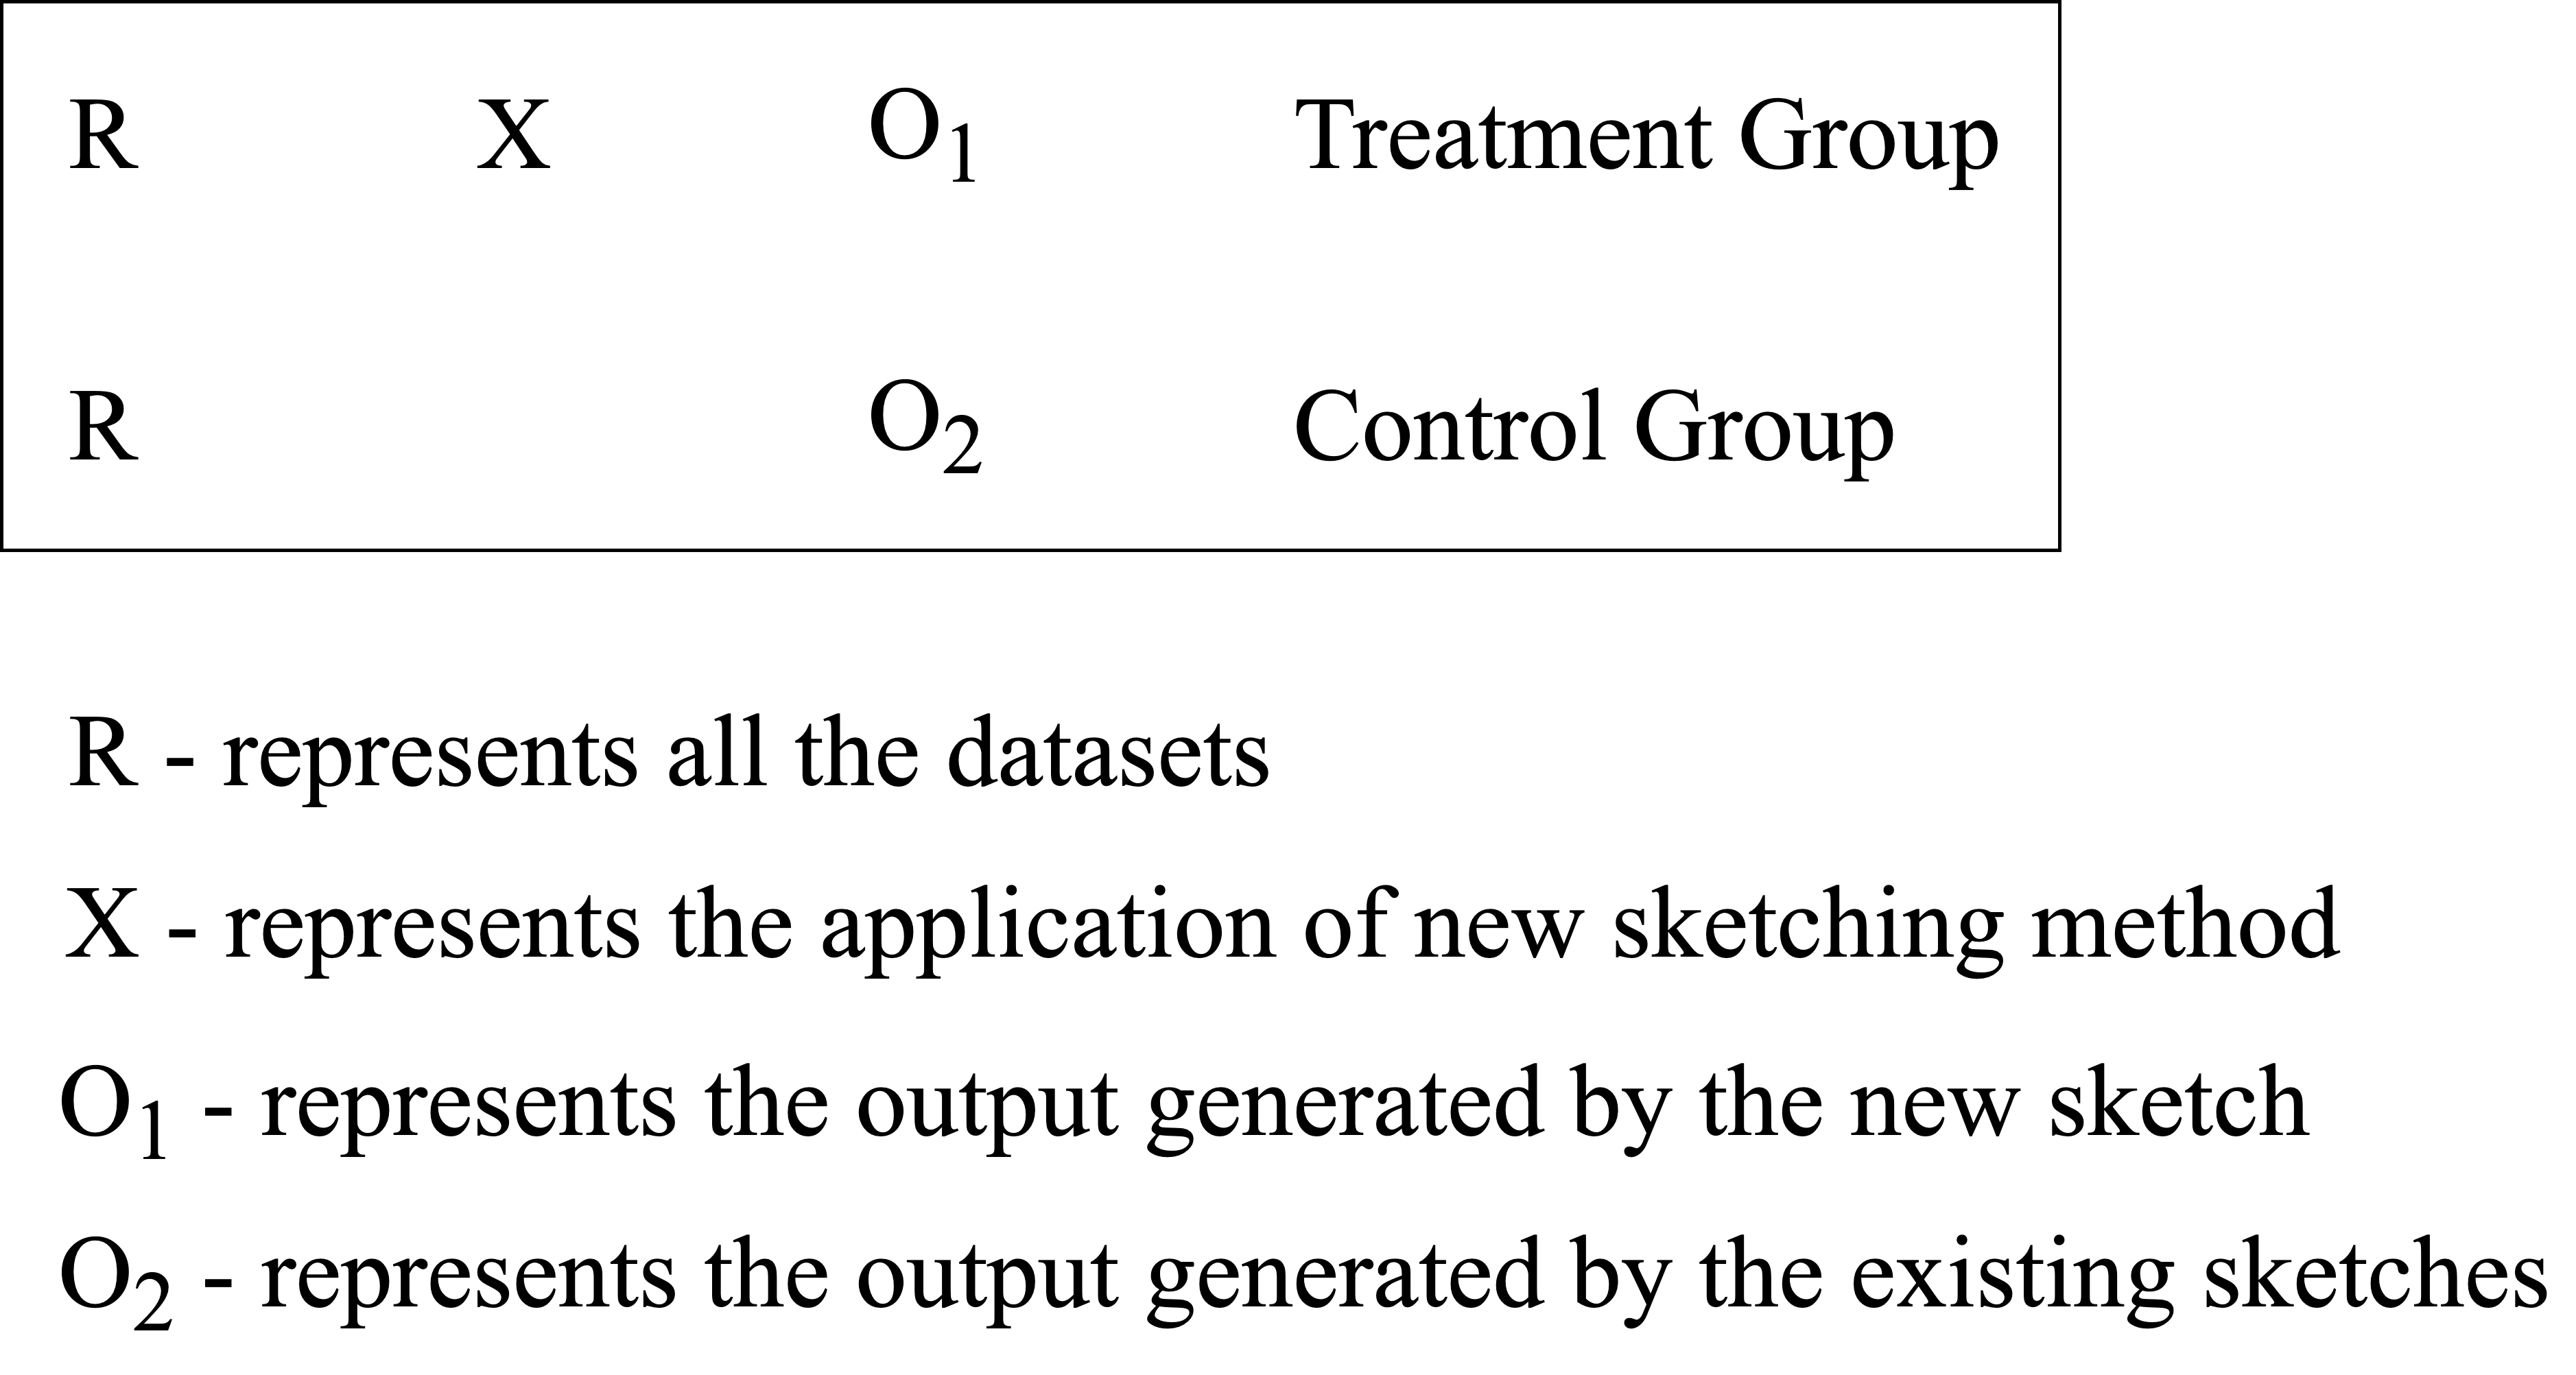
\includegraphics[width=0.6\textwidth]{images/design}
    \caption{Research design}
    \label{figure:design}
\end{figure}

\newpage
\chapter{Scope}

\section{In Scope}

\begin{enumerate}
    \item Project will improve upon the existing streaming graph sketching techniques. 
    \item Efficiency of running queries on various graph properties after the sketching process will be improved.
    \item New sketching techniques will be evaluated on a parallel framework.
\end{enumerate}

\section{Out of Scope}

\paragraph{}
There exists a number of methods for graph partitioning. The effect of these 
partitioning techniques will affect the results of the query efficiency and 
thus they will be considered during the experimentation phase and in presenting 
results. However no significant work or separate evaluation will be done with 
regard to graph partitioning. Improving partitioning techniques will be 
considered as out of scope for this research. 

\paragraph{}
Graph summarization could be mainly subdivided into Aggregation based, 
Attribute based, Compression and Application oriented. This research won’t 
explore the compression type graph summarization techniques. Much focus will 
be given to aggregation based sketching techniques. 

\paragraph{}
There are many security concerns with regard to the partitioning of streaming 
graphs and running sketching algorithms in a distributed environment. However 
the security aspects of sketch creation and partitioning will be considered 
as out of scope for this research as they are trivial to the holistic view 
of the research question, i.e, efficient sketching of streaming graphs. 

\newpage
\chapter{Timeline}

\section{Project Timeline}

\definecolor{bla}{rgb}{0.149, 0.196, 0.22}
\newcommand{\done}{\cellcolor{bla}}

\definecolor{lash}{rgb}{0.565, 0.643, 0.682}
\newcommand{\tbd}{\cellcolor{lash}}

\begin{table}[h]
    \begin{center}
        \begin{tabular}{ |p{0.5cm}|p{8cm}|p{0.2cm}|p{0.2cm}|p{0.2cm}|p{0.2cm}|p{0.2cm}|p{0.2cm}|p{0.2cm}|p{0.2cm}|p{0.2cm}|p{0.2cm}| } 
            \hline
            M & Milestone & \rotatebox[origin=c]{90}{ Feb } & \rotatebox[origin=c]{90}{Mar } & \rotatebox[origin=c]{90}{ Apr } & \rotatebox[origin=c]{90}{ May } & \rotatebox[origin=c]{90}{ Jun } & \rotatebox[origin=c]{90}{ Jul } & \rotatebox[origin=c]{90}{ Aug } & \rotatebox[origin=c]{90}{ Sep } & \rotatebox[origin=c]{90}{ Oct } & \rotatebox[origin=c]{90}{ Nov } \\
            \hline
            \multirow{3}{2em}{M1} & Research topic selection & \done & & & & & & & & & \\
            \cline{2-12}
            & Literature review & \done & \done & \done & \done & \done & \done & \done & \tbd & \tbd & \\
            \cline{2-12}
            & Draft the project proposal  & & \done & & & & & & & & \\
            \hline
            \multirow{3}{2em}{M2} & Preparing the test environment and the datasets & & & \done & & & & & & & \\
            \cline{2-12}
            & Implement the sketching algorithms & & & \done & & & & & & & \\
            \cline{2-12}
            & Initial evaluation & & & & \done & & & & & & \\
            \hline
            \multirow{2}{2em}{M3} & Propose improvements & & & & & \done & \done & \done & & & \\
            \cline{2-12}
            & Mid evaluation & & & & & \tbd & \tbd & \tbd & & & \\
            \hline
            \multirow{2}{2em}{M4} & Run on a parallel framework & & & & & & & & \tbd & & \\
            \cline{2-12}
            & Final evaluation & & & & & & & & \tbd & & \\
            \hline
            \multirow{2}{2em}{M5} & Writing the project thesis & & & & & & & & & \tbd & \tbd \\
            \cline{2-12}
            & Publication of the research & & & & & & & & & \tbd & \tbd \\
            \hline
        \end{tabular}
    \end{center}
    \caption{Timeline}
    \label{table:timeline}
\end{table}

\paragraph{}
According to the timeline indicated in Table \ref{table:timeline}, the research is in the M3 phase where improvements to the existing graph sketching techniques are proposed and benchmarked. 

\section{Progress so far}

\paragraph{}
The implementation will consist of,

\begin{itemize}
    \item Re-implementing the existing summarization techniques.
    \item Testing suite in order to benchmark the sketches. 
    \item Module stating the queries that needs to be executed during the benchmarking process. 
\end{itemize}

\paragraph{}
The modules that have been completed are indicated in Figure \ref{figure:progress}.

\begin{figure}[H]
    \centering
    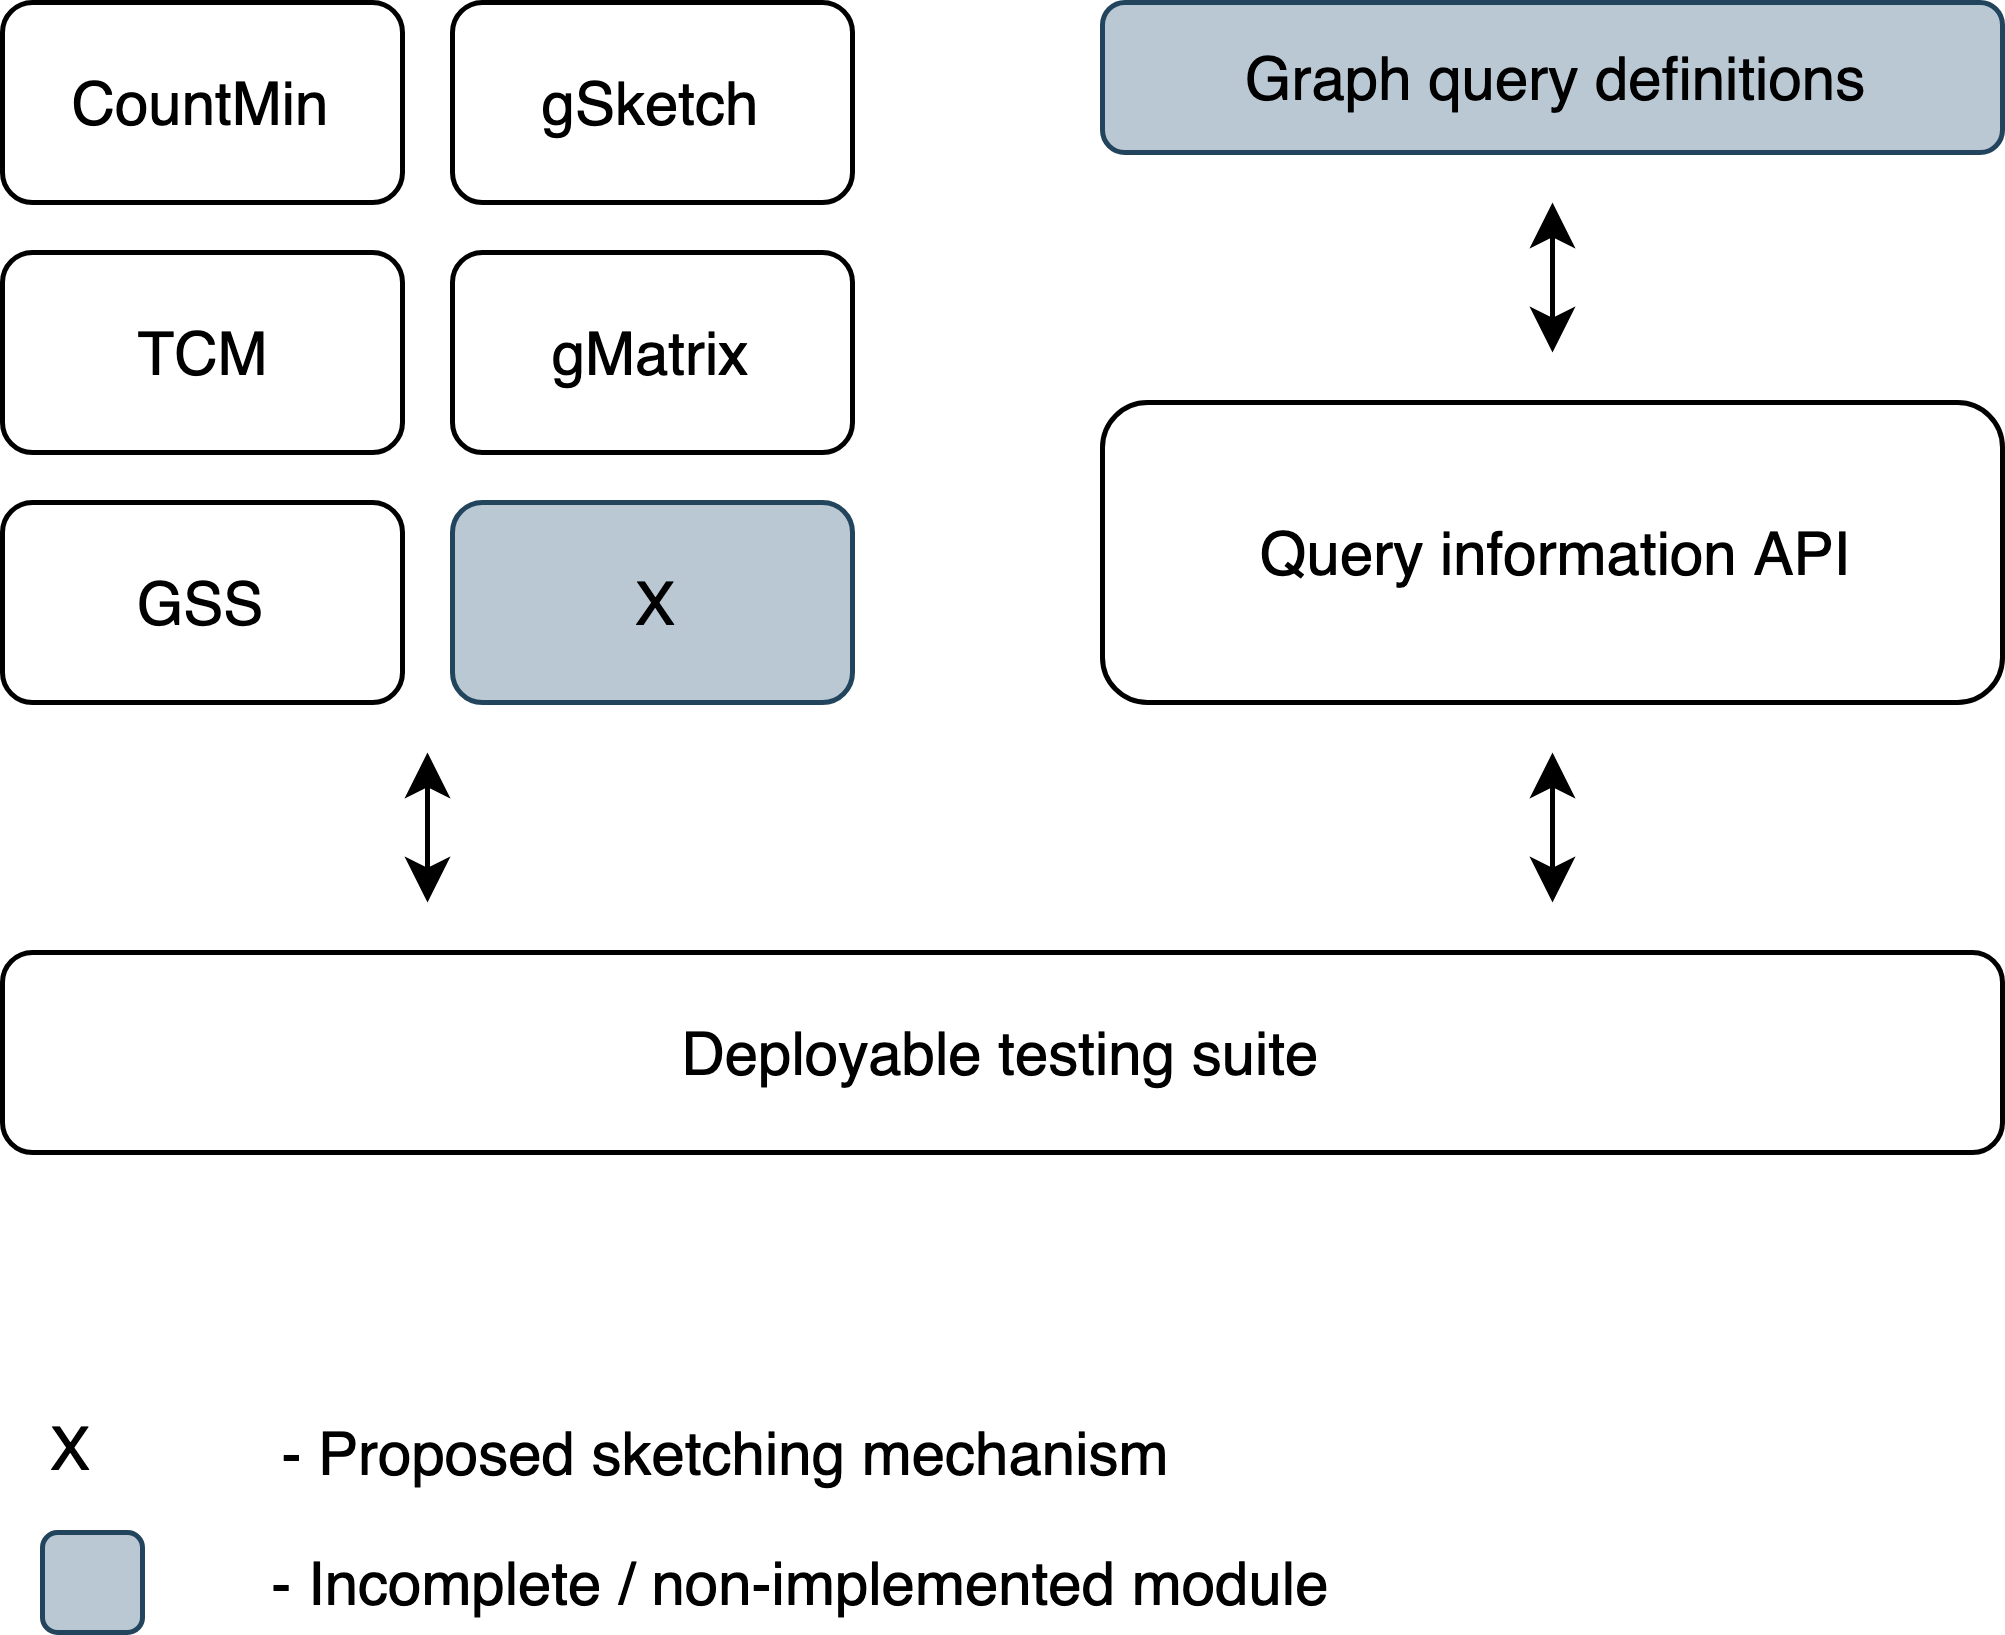
\includegraphics[width=0.7\textwidth]{images/progress}
    \caption{Overall progress}
    \label{figure:progress}
\end{figure}

\newpage
\chapter{Literature Review}

\paragraph{}
In this section we will give a review about theories and related work of this research. 

\section{Graphs in Real World}

\paragraph{}
Many real world datasets can be mapped into graphs. The users and the interactions between them, details about packet transfer in a computer network and a large citation database with authors of the research papers and their publications are some of the real world scenarios that could be mapped into graphs perfectly. Due to the sheer volume of the original datasets, the graphs produced from these datasets are also massive in size. 

\paragraph{}
Keeping these massive graphs in memory has become unrealistic with the large capacity that is required to store them. There are many challenges that lies in utilizing these graphs to derive knowledge through their properties while keeping them stored in secondary storage devices. This becomes easily evident in a scenario of a social network like Facebook or Twitter. Millions of user accounts interact with each other adding a large number of edges to the graph in a unit time. Retrieving the properties of this constantly evolving graph in realtime poses many difficulties. 

\paragraph{}
The properties of a graph that needs to be retrieved vary widely with the application scenario. In a social network it would be vital in finding the heavy hitter edges depicting the interaction between users or reachability of nodes showing how close the specific users are related. Model of a computer network would benefit with queries in finding heavy hitter nodes indicating possible destinations and sources of attacks originating within the network. Empirically, most real world graphs sparse and obey power law degree distribution. Most importantly, many of the real world scenarios get mapped into graph streams rather than static graphs. 

\section{Streaming Graphs}

\paragraph{}
Graphs can be divided into two as static graphs and streaming (dynamic) graphs. Static graphs are those which do not  change over time while streaming graphs are the ones which do get updated over time. These update operations could be insertion or deletion of nodes and edges. 

\paragraph{}
Determining the properties of streaming graphs is relatively strenuous than static graphs as they are constantly evolving. Usual graph algorithms cannot be run on streaming graphs due to their dynamic nature. Either the updating queries has to be stopped or a separate snapshot of the past should be used while running the graph algorithms. This is made even more difficult with the speed with which the graph is being updated. High throughput of update queries require any other types of queries to be run efficiently and as fast as possible in an unblocking manner. 

\paragraph{}
Real world streaming graphs could grow very large in size. Therefore these graphs are often stored as partitions in different machines over a network rather than in a single location. 

\section{Graph Partitioning}

\paragraph{}
The size of modern datasets has become too large to be fit into a single machine. It has become unrealistic to try to process the graphs mapped to these massive datasets while keeping them in the memory of a single node. Hence there exist a need to partition those large scale graphs into multiple machines. The communication between groups should be minimal to run graph algorithms on the whole graph effectively. However graph partitioning has been proved to be an NP-hard problem\cite{garey_simplified_1974}. Therefore the graph partitioning algorithms are only able to give sub-optimal solutions as of this date and thus a good streaming graph partitioning algorithm is impossible\cite{stanton_streaming_2012}. Graph partitioning algorithms can be mainly divided into two, such that, Online Graph Partitioning Algorithms and Offline Graph Partitioning Algorithms. The offline partitioning algorithms such as METIS\cite{karypis_fast_1998}, Chaco\cite{hendrickson_chaco_1993}, SBV-cut\cite{kim_sbv-cut:_2012} need to load the entire graph into the memory for the algorithm to be run. But the online partitioning algorithms like PreferBig\cite{stanton_streaming_2012} and HoVerCut\cite{sajjad_boosting_2016} keeps a buffer of the edge streams and process them when the buffer gets full. 

\section{Graph Summarization}

\paragraph{}
Reducing the complexity of a graph while retaining some of its original properties is known as graph summarization. These summaries often incur an error when running algorithms due to the loss of information. But usually when it comes to real world massive graphs such as social networks, it is enough to obtain approximations instead of the exact answers with reduced computational cost. Graph summarization has a wide range of benefits including reduction of data volume and storage, speedup of graph algorithms and queries, interactive analysis support and noise elimination\cite{liu_graph_2018}.  

\paragraph{}
There are many challenges involving in graph summarization. Dealing with the sheer volume of data might prove to be a cumbersome task due to memory limitations. The sketch also has to deal with the complexity of the data because real world graphs are sometimes heterogeneous. Summarization deals with extracting interesting information out of a graph. However the definition of interesting might vary depending on the application. Furthermore the evaluation of graph summaries present additional challenges as it depends on the application domain. Change over time is also a challenge when dealing with graph summarization. Graphs change over time and their summaries should be changed as well. Efficient methods should be devised in order to add the changes to the existing summaries. 

\paragraph{}
There are few core techniques used when summarizing graphs\cite{liu_graph_2018}.
\begin{itemize}
    \item Grouping or aggregation based
    \item Bit compression based
    \item Simplification or sparsification based
    \item Influence based
\end{itemize}

\paragraph{}
Graphs are summarized with different intentions. One of the main considerations is to compress the graph so that it occupies less space in memory. Another objective could be for the ease of visualization. It is much more practical to visualize a smaller graph rather than one containing millions of nodes. Sometimes summarization is done with security in mind, in order to remove sensitive information from the original dataset. But during this research our aim lies in query optimization through summarization. 

\subsection{Streaming Graph Summarization}

\paragraph{}
Summarizing graph streams is more difficult than summarizing a static graph due to the constant flow of data. Underlying original graph is constantly updated while it is being summarized. Therefore the summarization process has to be done in realtime. Almost any static graph summarization technique could be used with streaming graph snapshots within specific time frames. However keeping time snapshots of data could very well be an unrealistic goal in a massive streaming graph. Thus sophisticated sparsification techniques have to be derived in order to summarize streaming graphs. 

\section{Related Work}

\paragraph{}
Restating the aforementioned, we are concerned with graph summarization techniques which mainly aim in preserving query efficiency after summarization during this research. 

\subsection{CountMin}

\begin{figure}[H]
    \centering
    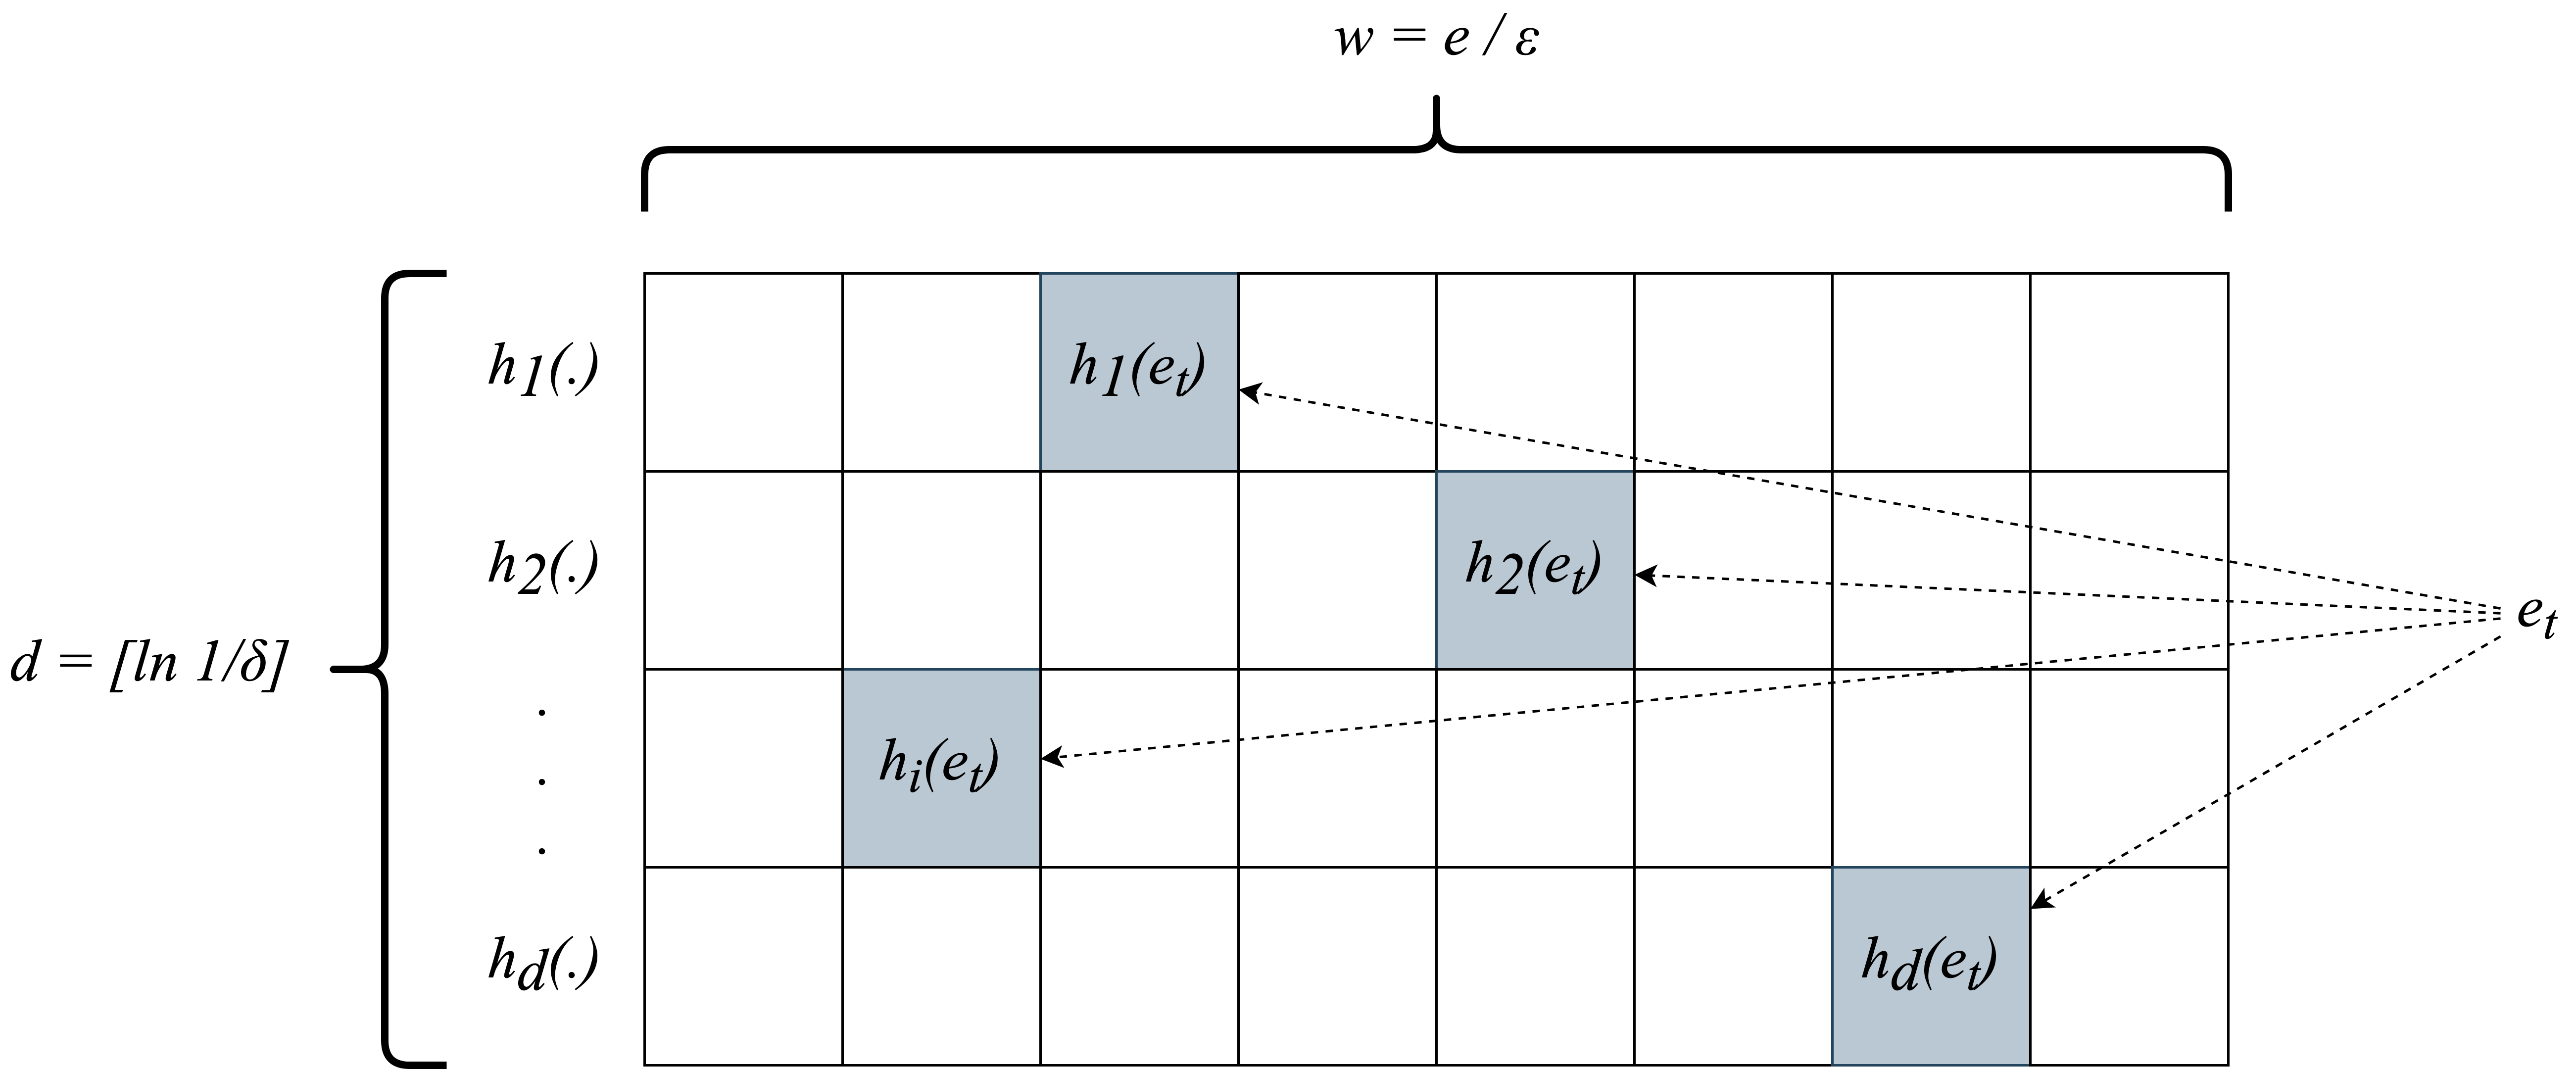
\includegraphics[width=0.9\textwidth]{images/countmin}
    \caption{CountMin sketch}
    \label{figure:countmin}
\end{figure}

\paragraph{}
CountMin\cite{cormode_improved_2003} could be considered as the pioneering work in summarizing data streams which are directly related to our research. CountMin\cite{cormode_improved_2003} is a data structure that is used for frequency approximation queries. The underlying idea behind the CountMin\cite{cormode_improved_2003} data structure is to hash the aggregated frequencies of the edges using multiple hash functions into predefined blocks as indicated in Figure \ref{figure:countmin}. A fixed sized will be stated at the time of creation of the CountMin\cite{cormode_improved_2003} sketch and irrespective of the volume of data stored, the size of the sketch does not have to be changed. The major drawback in following this procedure is that the error of the queries reduce as more and more data is introduced to the sketch. However despite these weaknesses, CountMin\cite{cormode_improved_2003} can be considered as a good generalized sketch at the time as many other sketches described in the literature are good for one single pre-specified aggregate computation. Therefore CountMin\cite{cormode_improved_2003} approach is not restricted to streaming graphs but other applications as well\cite{cormode_improved_2003}. 

\subsection{gSketch}

\paragraph{}
gSketch\cite{zhao_gsketch:_2011} is an extension of CountMin\cite{cormode_improved_2003} data structure. But unlike CountMin\cite{cormode_improved_2003} sketch, this is specifically geared towards summarizing graph streams. gSketch\cite{zhao_gsketch:_2011} is based on one of the two assumptions that,

\begin{enumerate}
    \item A graph stream sample is available.
    \item Both graph stream sample and a query workload sample are available.
\end{enumerate}

\begin{figure}[H]
    \centering
    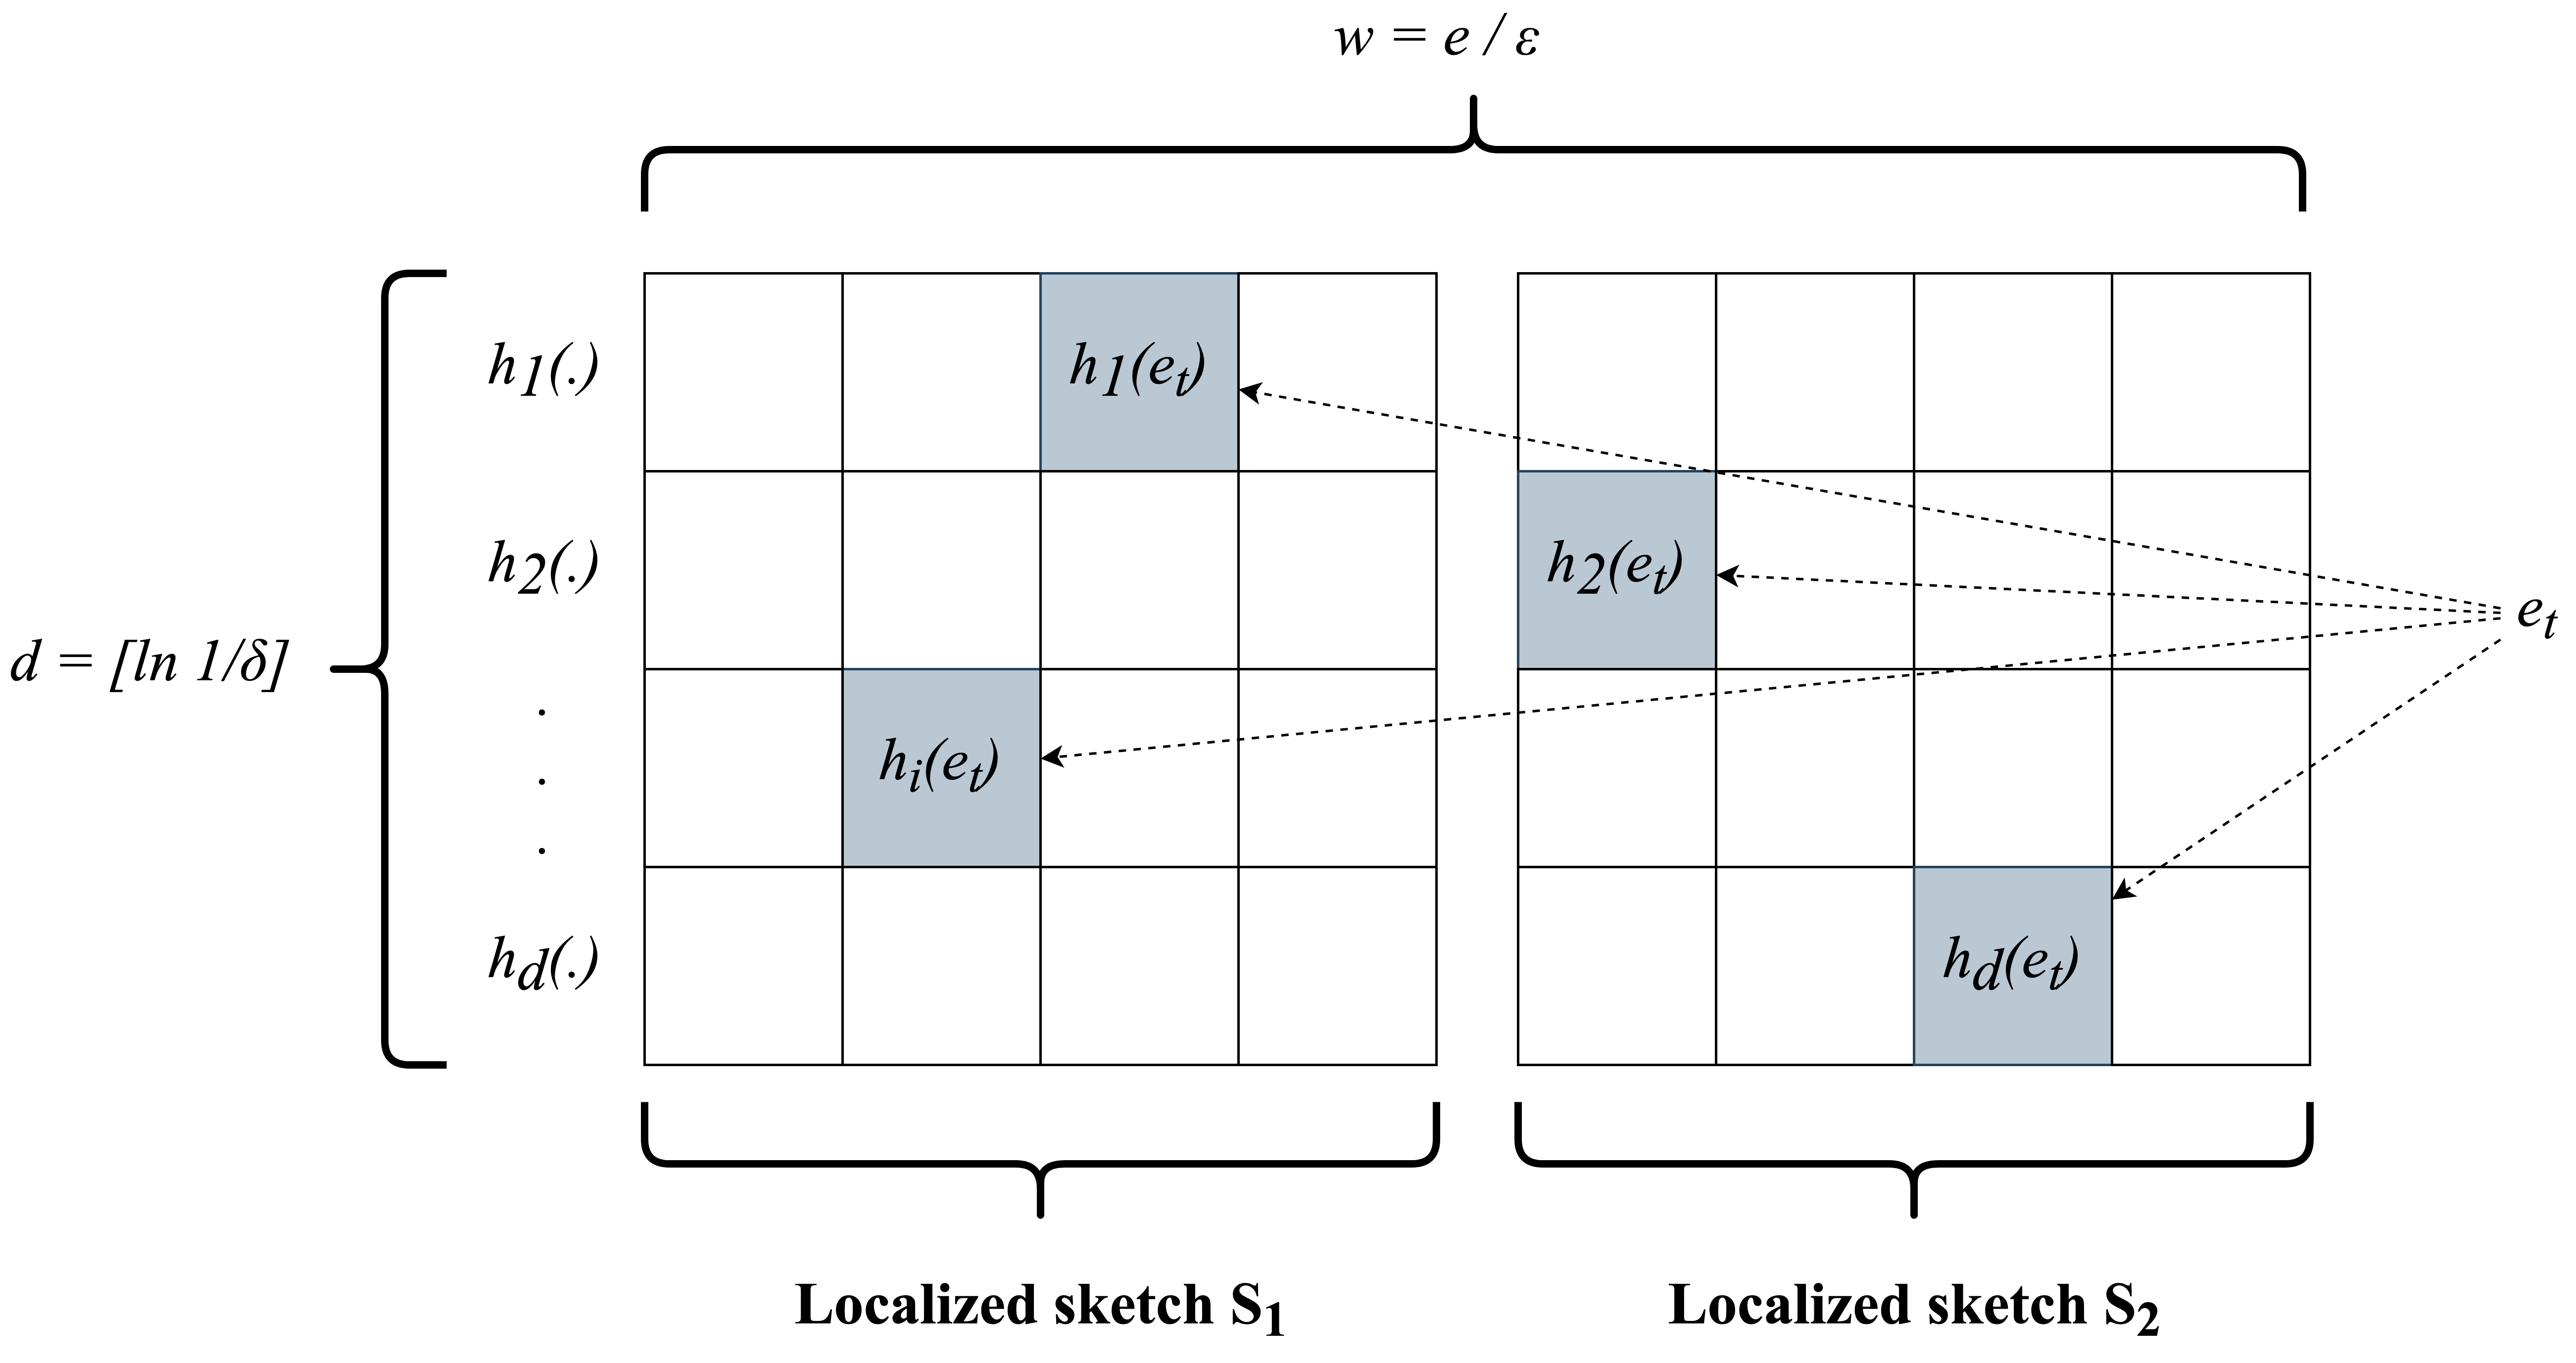
\includegraphics[width=0.9\textwidth]{images/gsketch}
    \caption{gSketch}
    \label{figure:gsketch}
\end{figure}

\paragraph{}
As per the previous sketching technique, CountMin\cite{cormode_improved_2003}, a global sketch is created for the entire graph stream. The disadvantage of this method is that any structural properties present in the graph stream are completely ignored throughout this process. gSketch\cite{zhao_gsketch:_2011} tries to avoid by considering the underlying structural properties of the graph. 

\paragraph{}
The specialty of gSketch\cite{zhao_gsketch:_2011} is to pre-process the stream samples and creating sketch partitions as indicated in Figure \ref{figure:gsketch}. Its goal is to maintain sufficient frequency uniformity within each localized sketch so that the query estimation can be optimized over the entire graph stream. 

\subsection{TCM}

\begin{figure}[H]
    \centering
    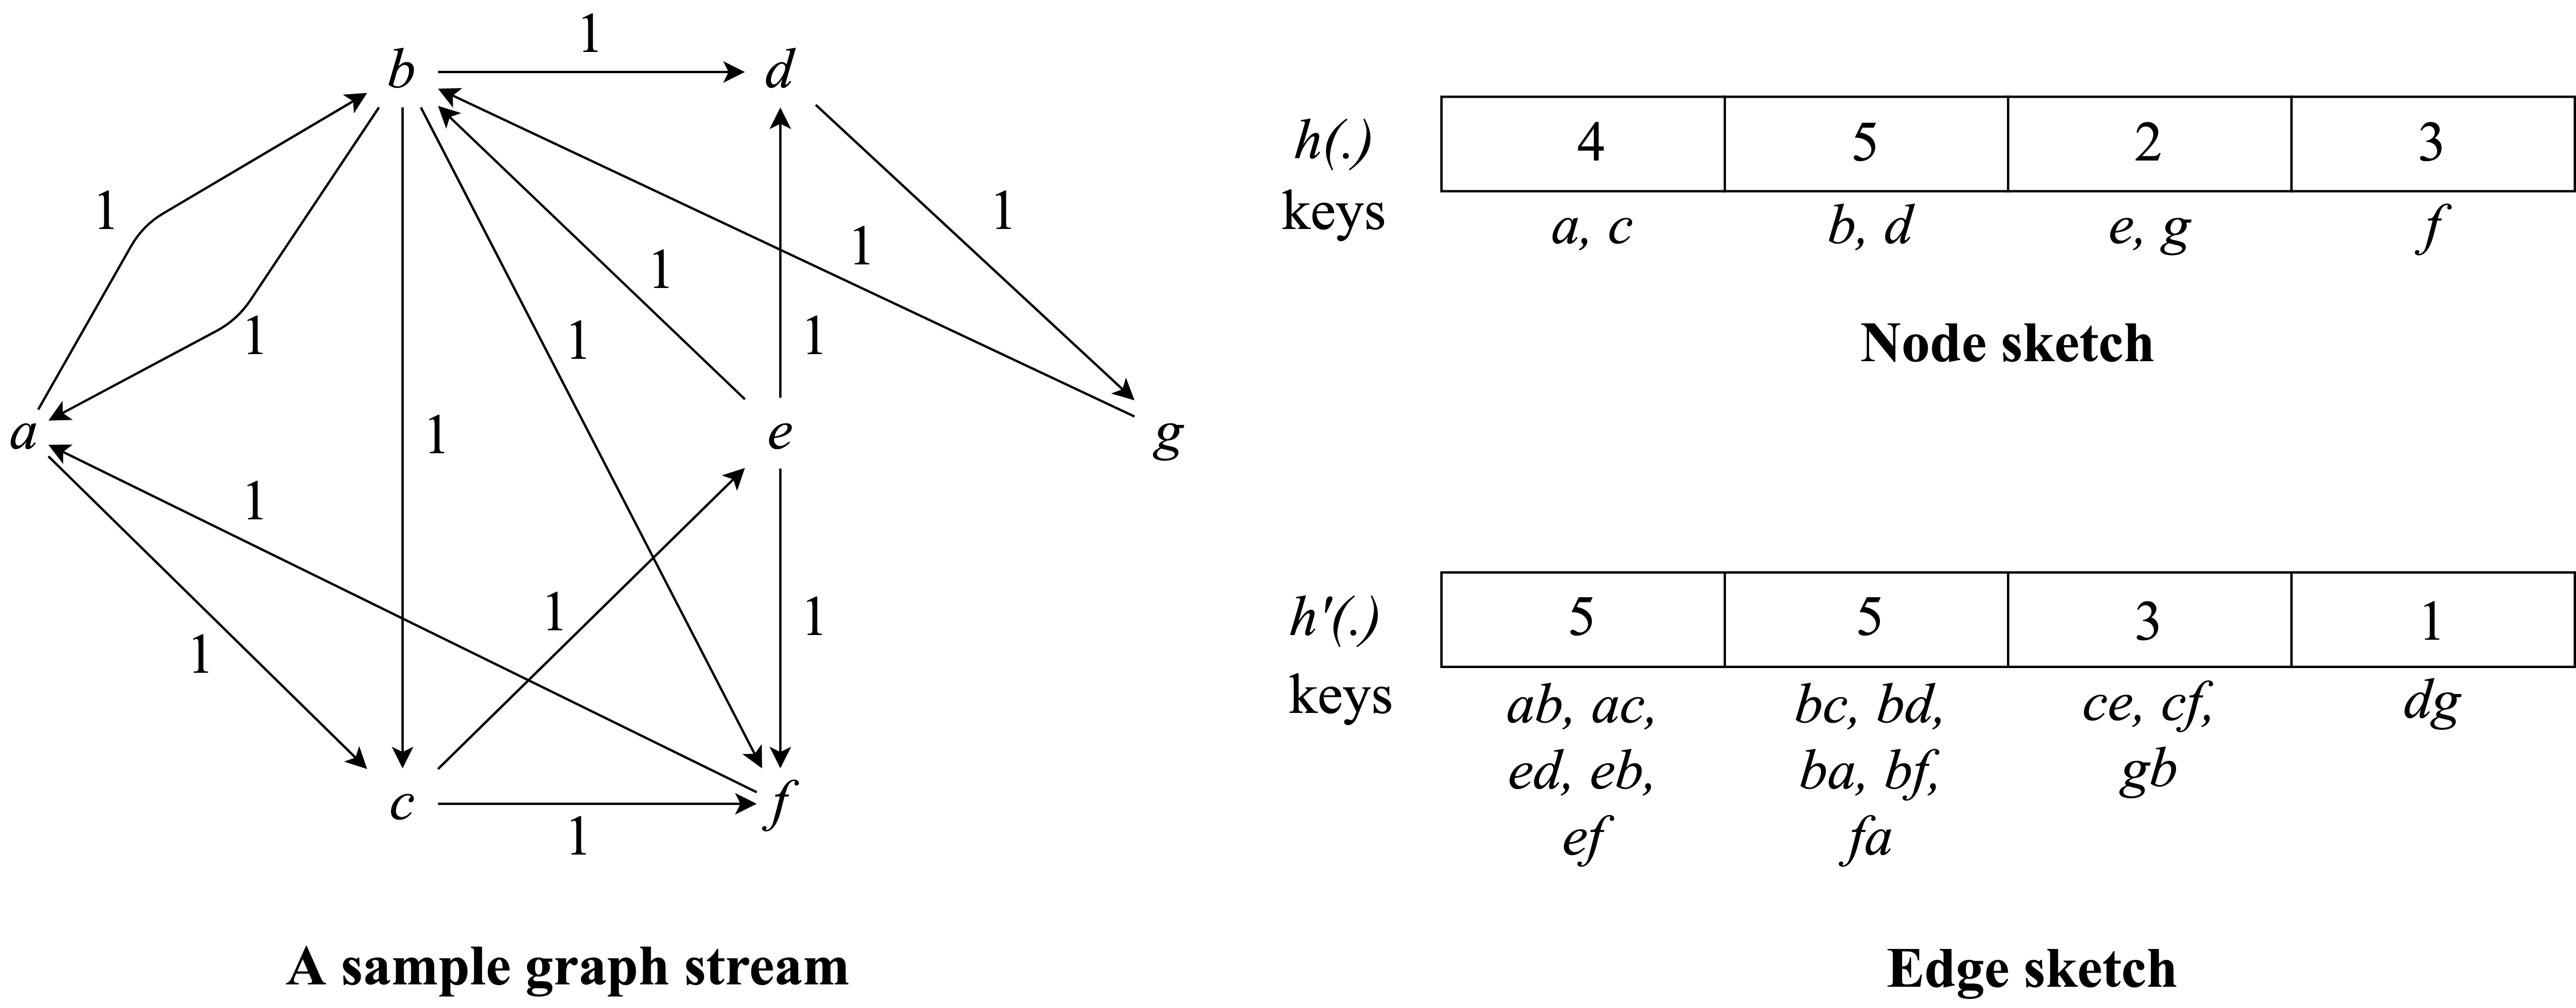
\includegraphics[width=\textwidth]{images/approximate_frequency_counts}
    \caption{Approximate Frequency Counts}
    \label{figure:afc}
\end{figure}

\paragraph{}
Approximate Frequency Count sketches store aggregated frequencies of edges in summarized form as shown in the example in Figure \ref{figure:afc}.

\paragraph{}
A disadvantage posed by all the approximate frequency count sketches like CountMin\cite{cormode_improved_2003} or gSketch\cite{zhao_gsketch:_2011} is that they do no store the locality of the nodes. Therefore they cannot be used for conditional node queries or queries involving node connectivity. If these queries were to be run, at least some of the information about the locality of nodes has to be retained in the graph synopses. TCM\cite{tang_graph_2016} can summarize both node and edge information in constant time. Because of that it can answer a wide range of queries unlike its predecessors. The structure of a TCM sketch is depicted in Figure \ref{figure:tcm}.

\begin{figure}[H]
    \centering
    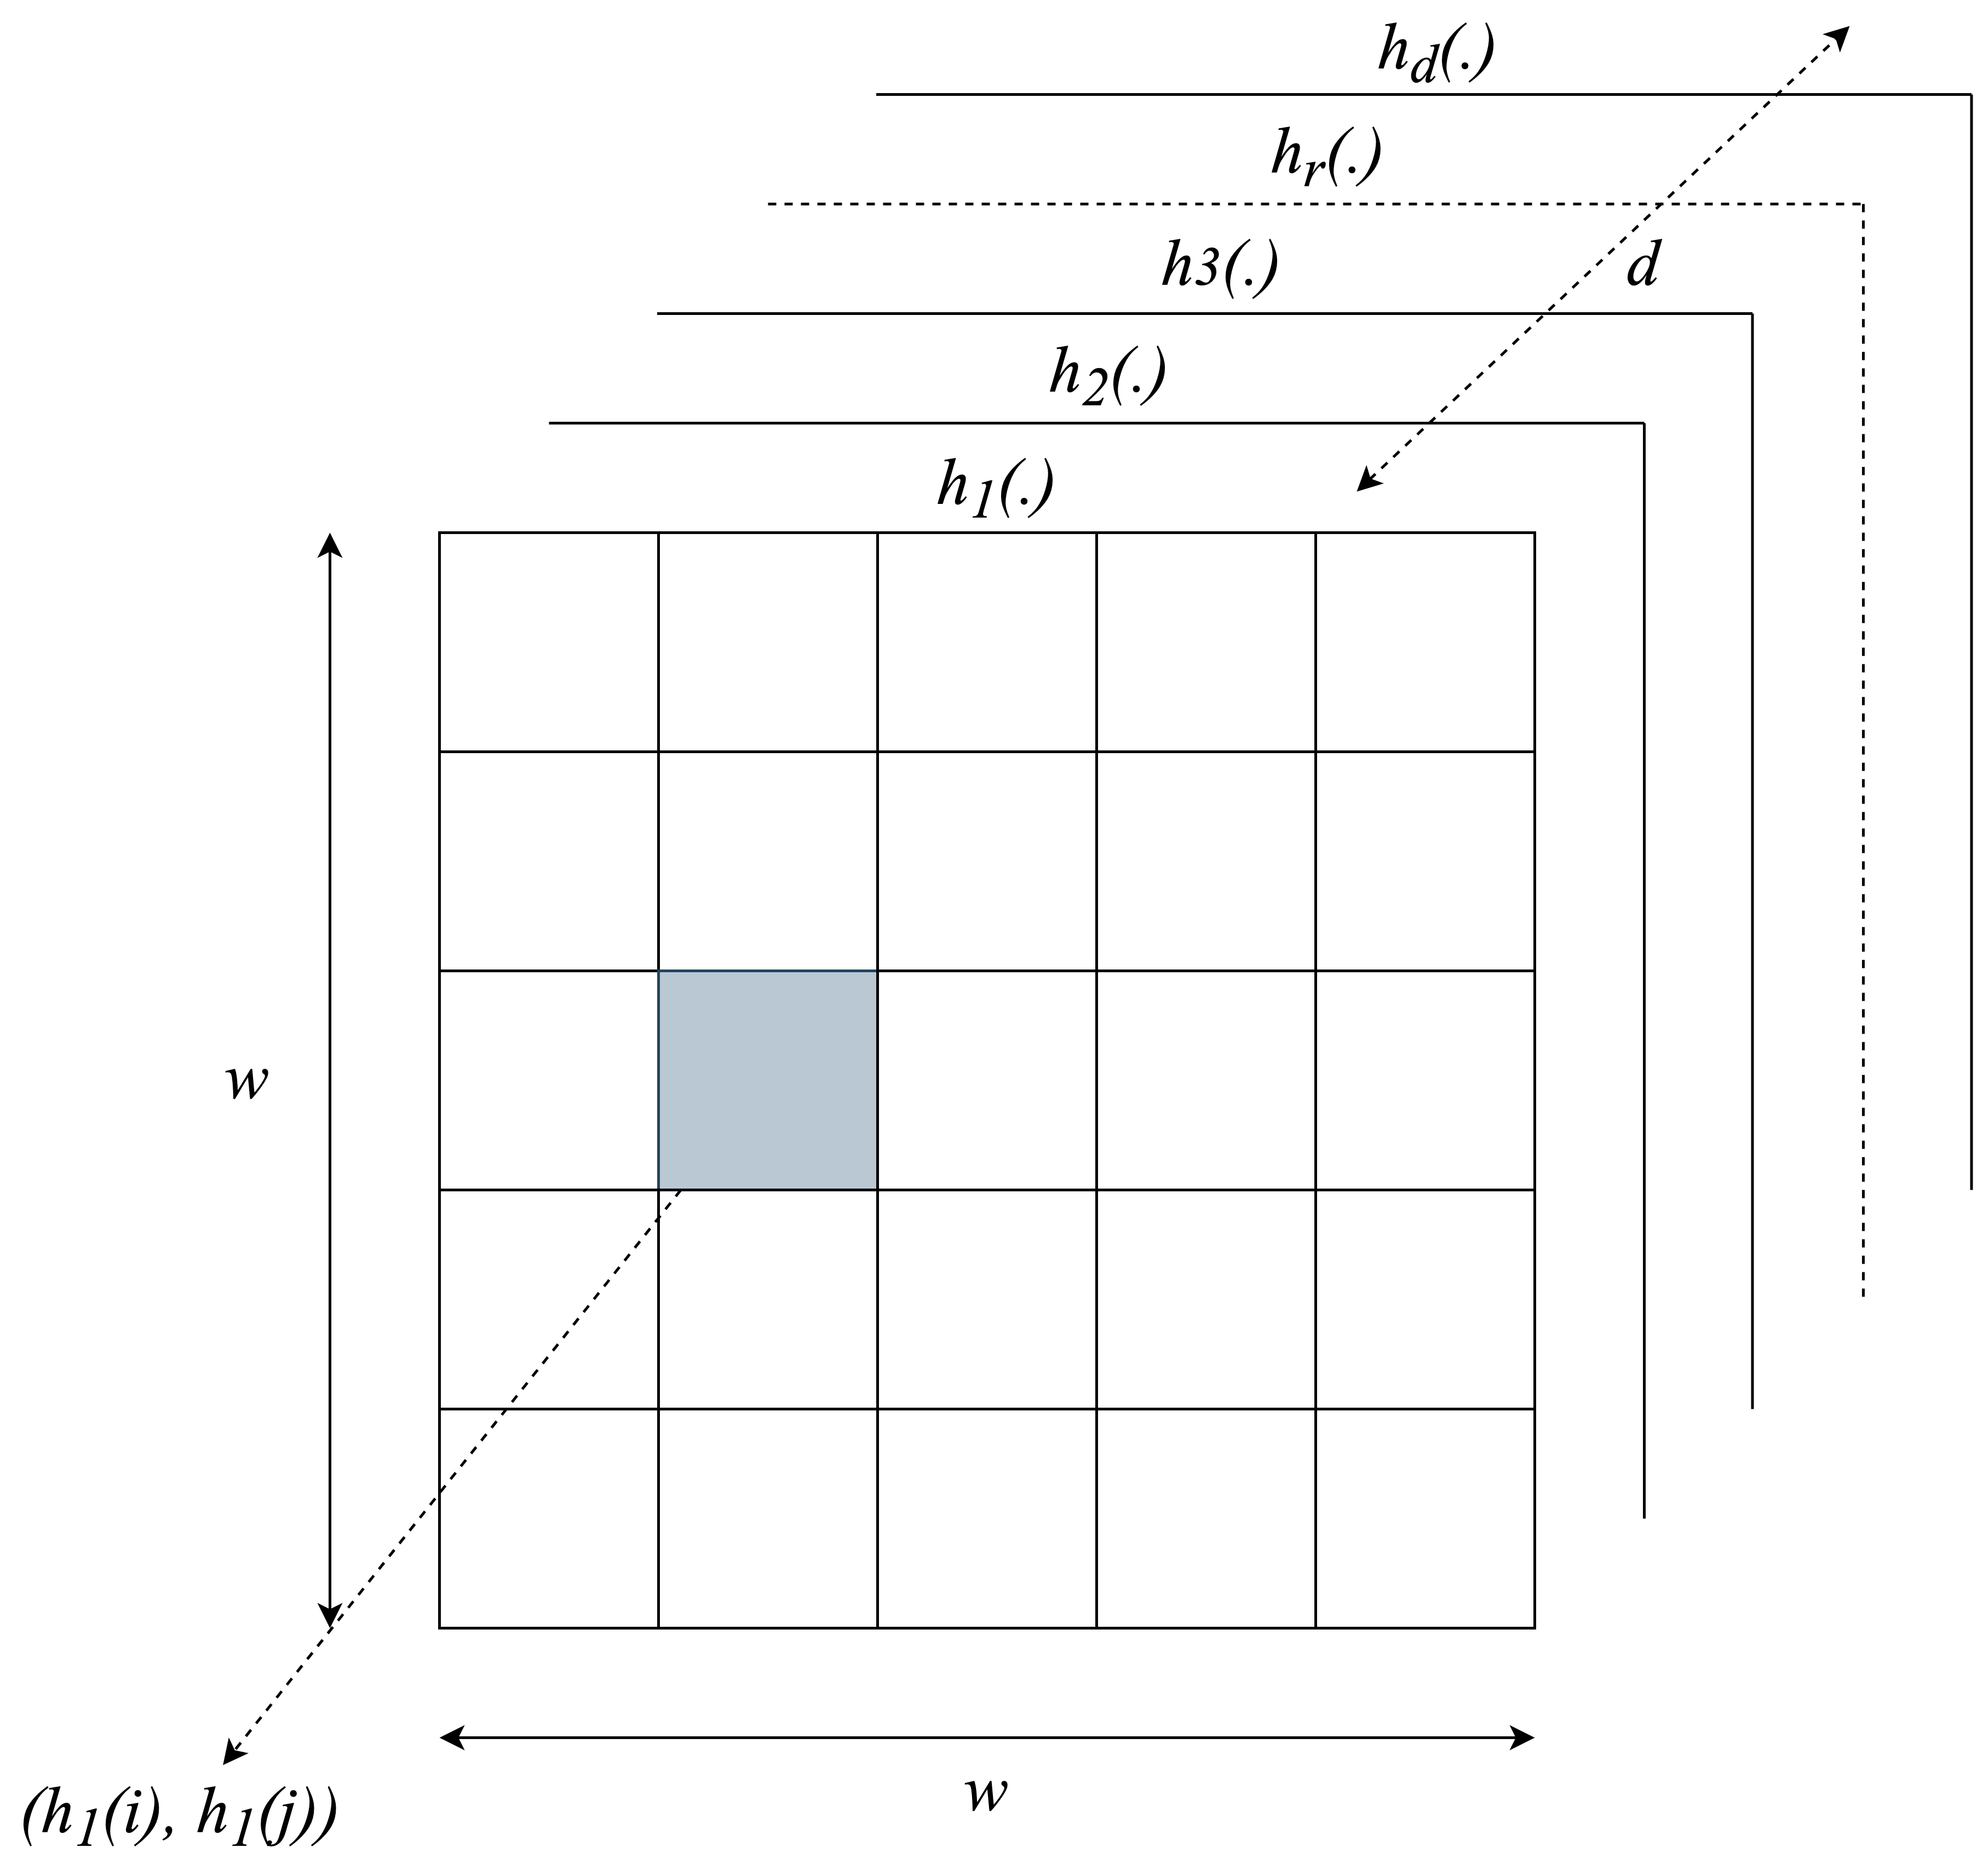
\includegraphics[width=0.5\textwidth]{images/tcm}
    \caption{TCM}
    \label{figure:tcm}
\end{figure}

\subsection{gMatrix}

\paragraph{}
gMatrix\cite{khan_query-friendly_2016} is a very similar to TCM and it was proposed in the same year as the TCM. However gMatrix\cite{khan_query-friendly_2016} paper consider about,

\begin{itemize}
    \item reverse hashing queries through pairwise independent hash functions;
    \item alternative options to extend sketch and space-saving synopses for achieving similar functionalities as gMatrix\cite{khan_query-friendly_2016};
\end{itemize}

which the TCM paper does not address. 

\subsection{GSS}

\paragraph{}
GSS\cite{gou_fast_2018} is the latest graph summarization technique that has been introduced up to date which was published in 2018. Even when using 1/256 memory size of the state of the art graph summarization algorithm, GSS\cite{gou_fast_2018} still significantly outperformed it for most queries\cite{gou_fast_2018}. The GSS paper\cite{gou_fast_2018} points out that even if TCM\cite{tang_graph_2016} and gMatrix\cite{khan_query-friendly_2016} supports all queries in the streaming graphs in contrast to CM sketches\cite{cormode_improved_2003} and gSketches\cite{zhao_gsketch:_2011} which only supports queries for edges and do not get involved with the topology of the underlying graph, they suffer from poor accuracy. GSS\cite{gou_fast_2018} improves upon TCM\cite{tang_graph_2016} and gMatrix\cite{khan_query-friendly_2016} to increase the accuracy with less memory usage. 

\paragraph{}
GSS\cite{gou_fast_2018} defines three graph primitives as,

\begin{itemize}
    \item Edge query 
    \item 1-hop Successor query 
    \item 1-hop Precursor query
\end{itemize}

By supporting all these 3 types of queries it is possible to reconstruct the entire graph. Therefore it is also possible to run any kind of query against a sketch which supports all 3 of the above primitives. 

\paragraph{}
The intuition behind the basic version of the GSS\cite{gou_fast_2018} can be illustrated as below. 

\begin{figure}[H]
    \centering
    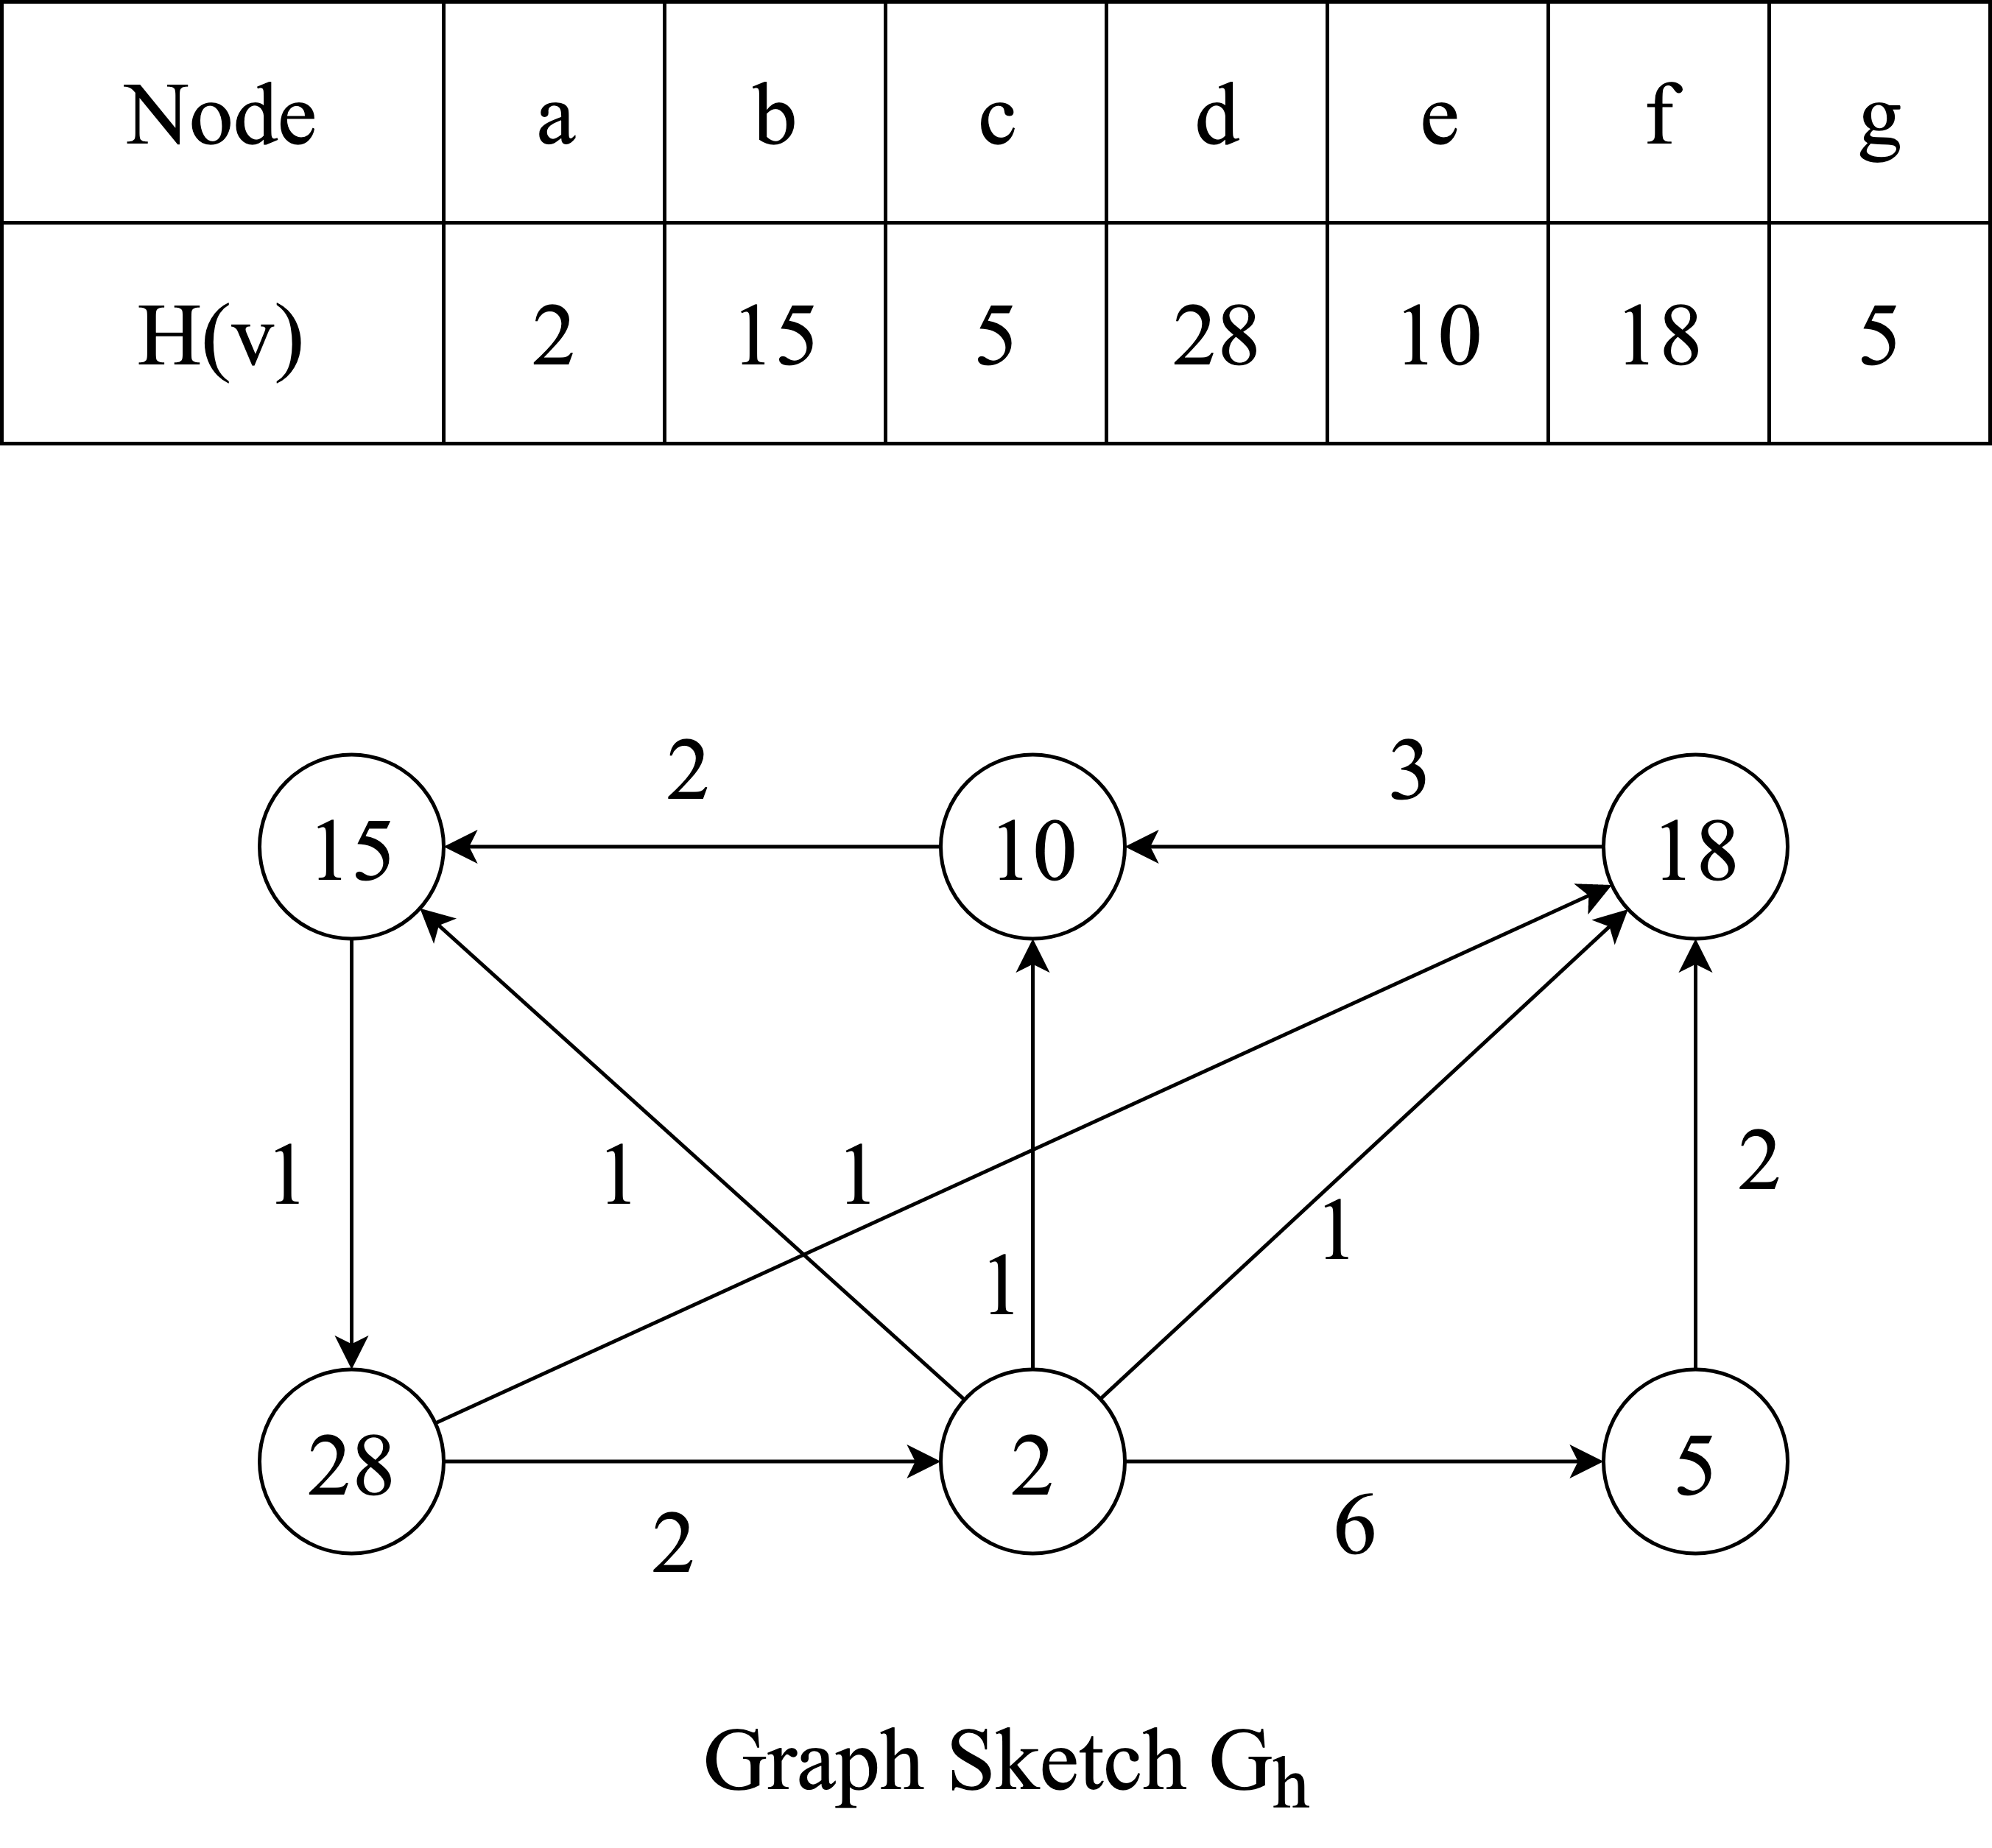
\includegraphics[width=0.5\textwidth]{images/gss1}
    \caption{A sample map function\cite{gou_fast_2018}}
    \label{figure:gss1}
\end{figure}

\paragraph{}
\(H(.)\) is a hash function which is used on the vertices of the original graph stream to create the graph sketch \(G\textsubscript{h}\) as indicated in Figure \ref{figure:gss1}.

\paragraph{}
A GSS\cite{gou_fast_2018} sketch consists of two parts, 

\begin{itemize}
    \item An \(m \times m\) adjacency matrix
    \item List buffer B for leftover edges
\end{itemize}

\paragraph{}
For each node in the sketch graph \(G\textsubscript{h}\), an address \(h(v)\) and a fingerprint \(f(v)\) is defined. Each edge \(H(s)\), \(H(d)\) is mapped into a bucket in the row \(h(s)\), column \(h(d)\) of the matrix. \([\langle f(s), f(d)\rangle, w]\) is recorded in the corresponding bucket of the matrix, where \(w\) is the edge weight and \(f(s)\), \(f(d)\) are the fingerprints for the source and destination. This can be seen in the sample of GSS sketch shown in Figure \ref{figure:gss2}.

\begin{figure}[H]
    \centering
    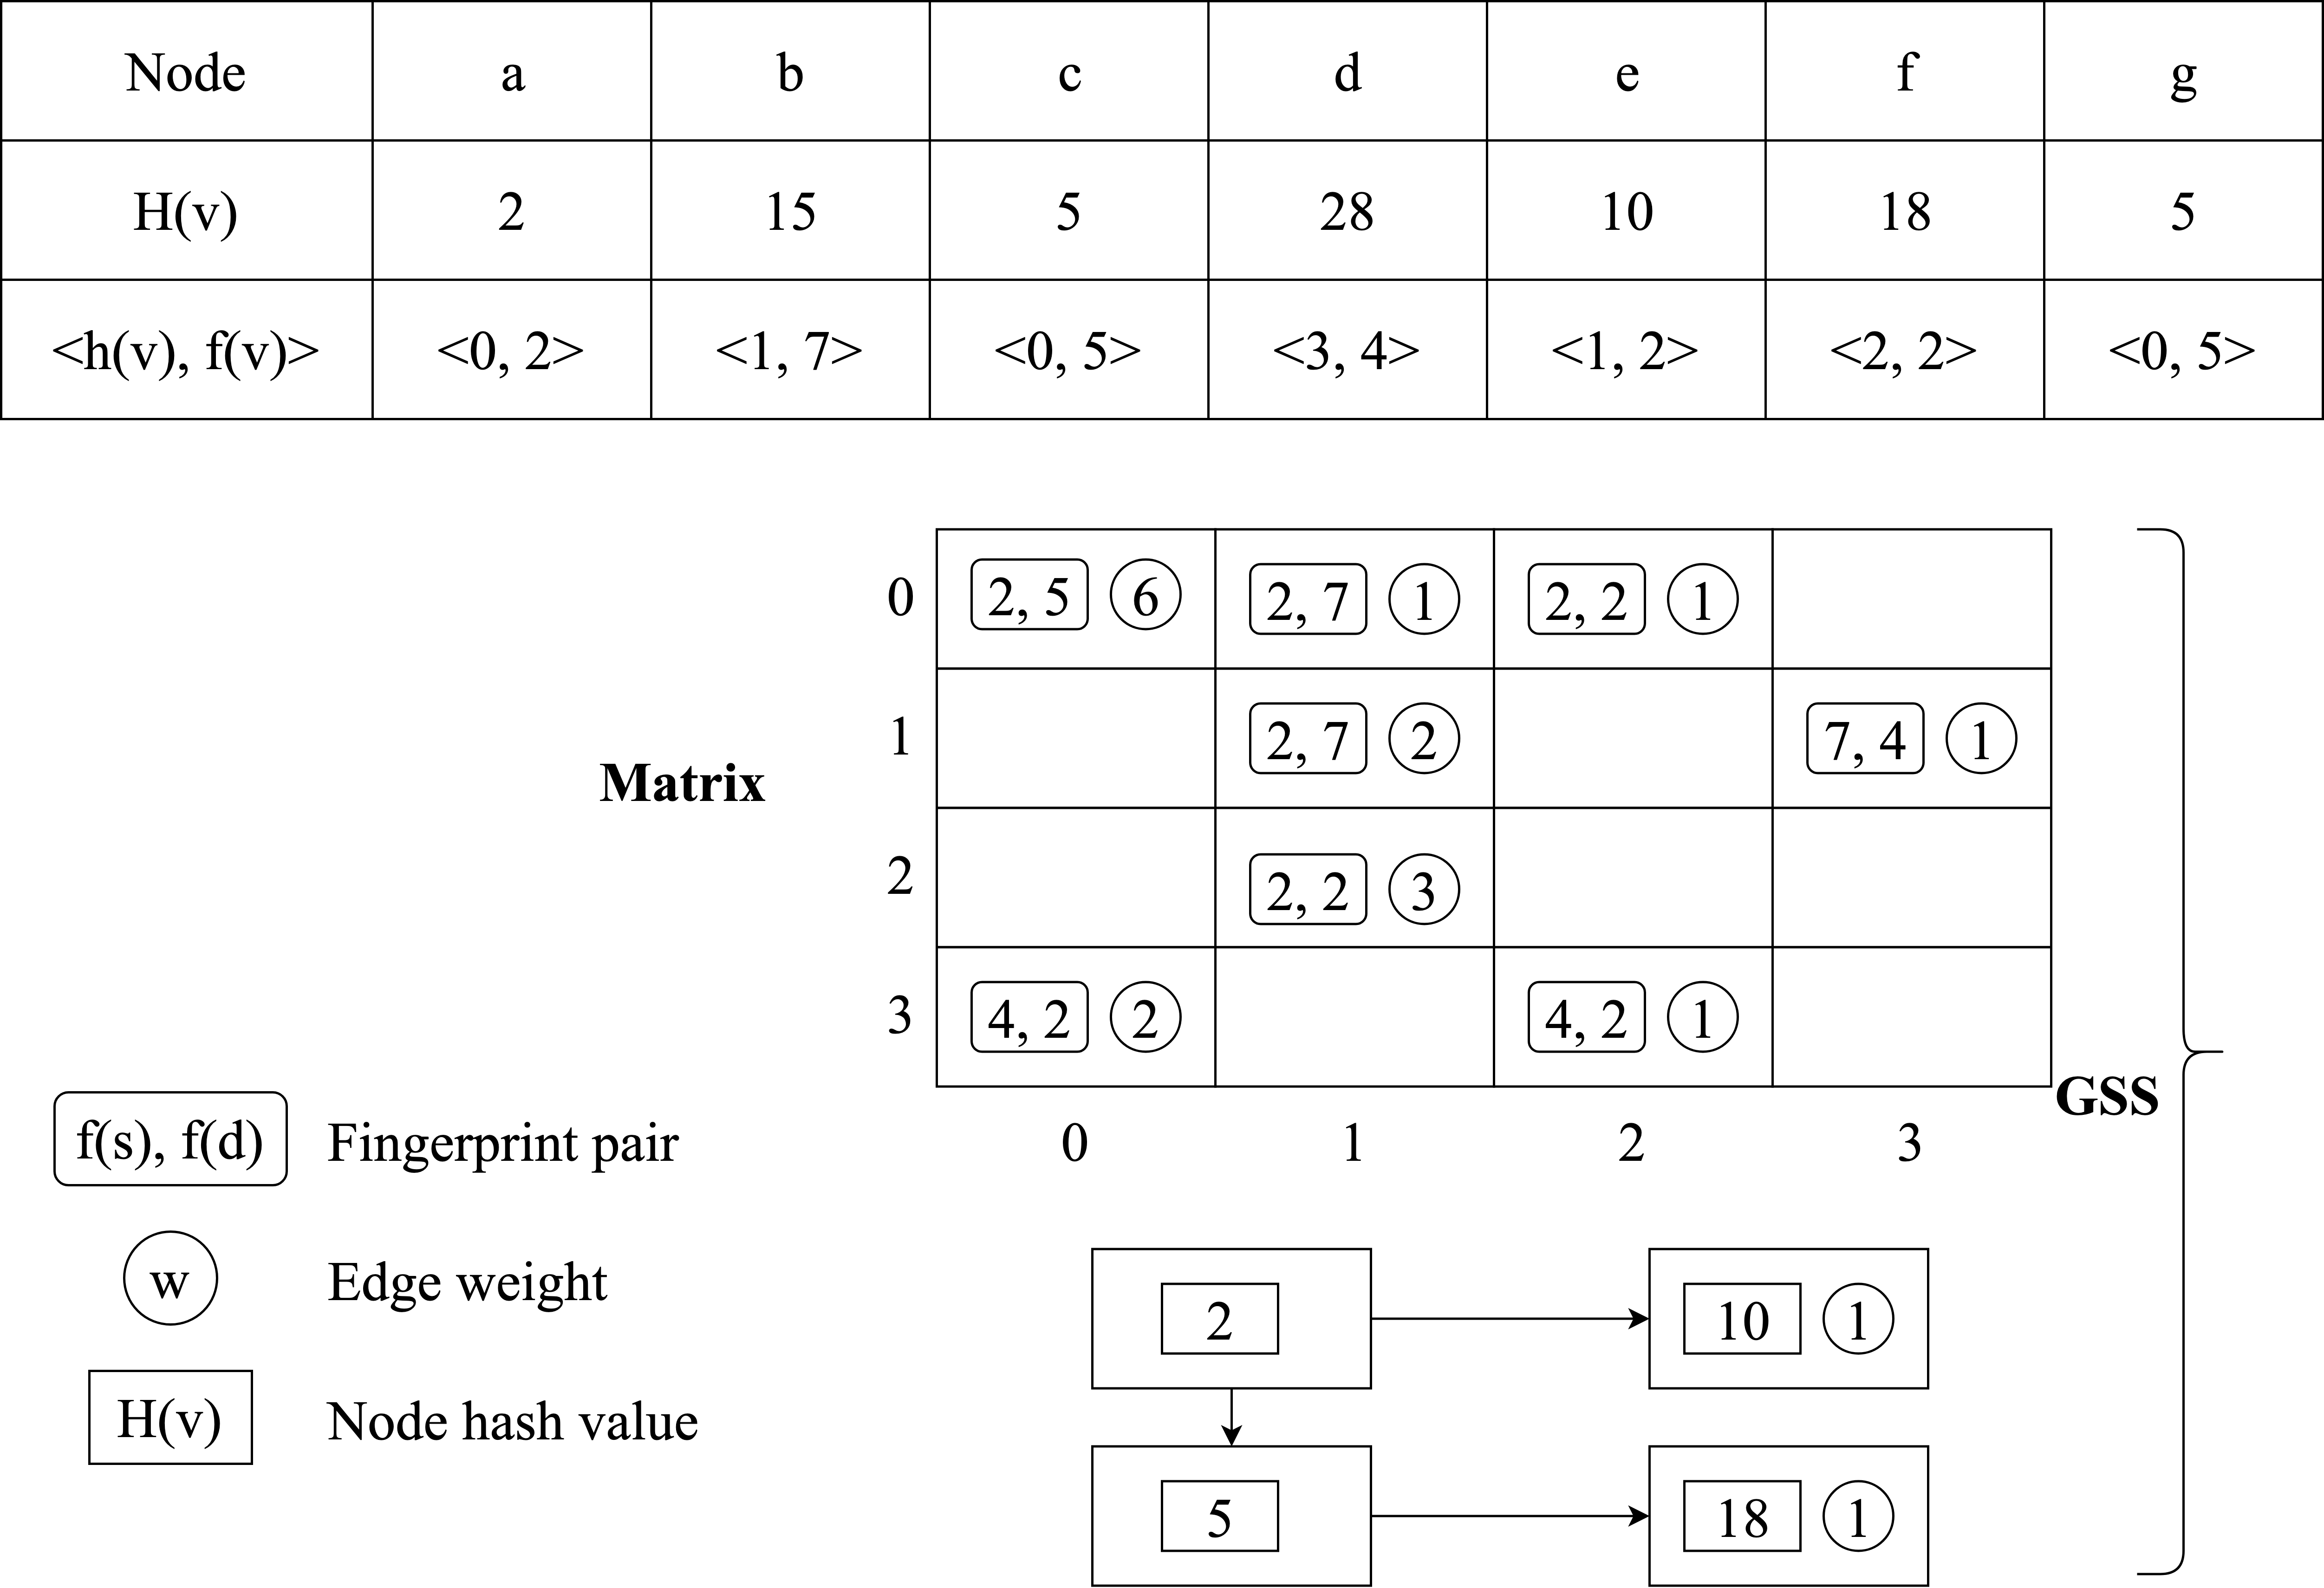
\includegraphics[width=0.9\textwidth]{images/gss2}
    \caption{A sample version of the basic data structure\cite{gou_fast_2018}}
    \label{figure:gss2}
\end{figure}

% \section{Summary}

% \paragraph{}
% Some summary----

\newpage
\chapter{Research Design}

\paragraph{}
Our research design has been further refined after the initial design to ensure that the plan for the research helps in properly answering the research questions. High level diagram for the research design is shown in Figure \ref{figure:des}.

\begin{figure}[H]
    \centering
    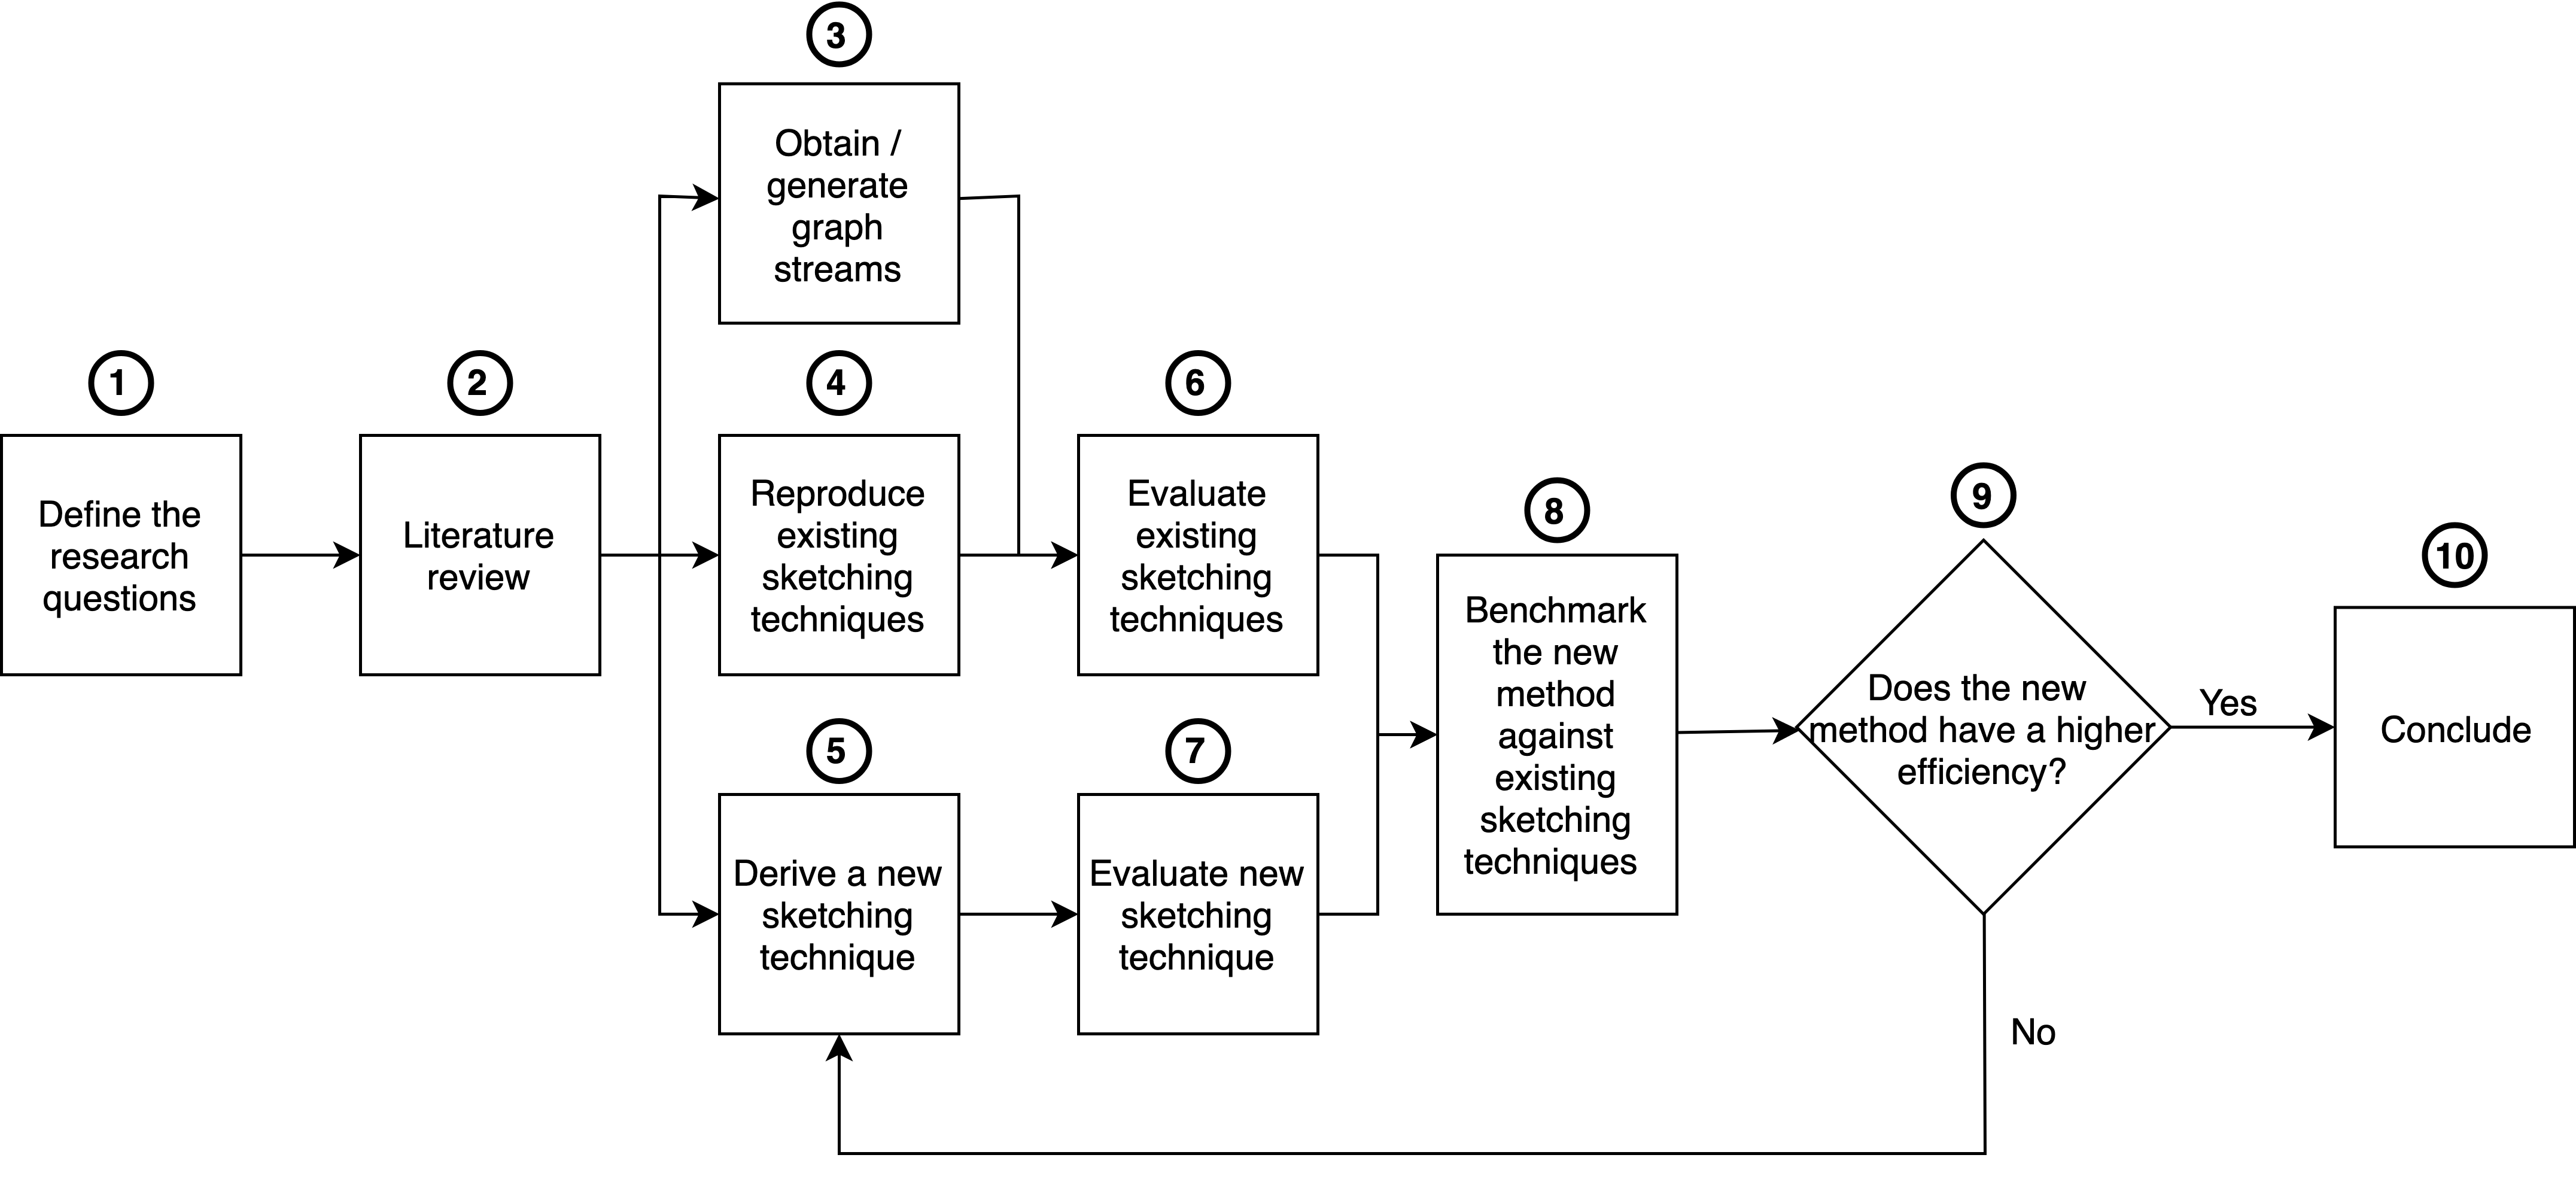
\includegraphics[width=\textwidth]{images/research-design}
    \caption{High level diagram of the research design}
    \label{figure:des}
\end{figure}

\section*{Step 1 - Define the research question}

\paragraph{}
Our research question is,

\begin{itemize}
    \item How to improve upon existing streaming graph sketching techniques such that the graph properties could be identified in realtime? 
\end{itemize}

\paragraph{}
In order to achieve this, a comprehensive literature review on the existing streaming graph sketching techniques would have to be done. This will be done in step 2. 

\section*{Step 2 - Literature review}

\paragraph{}
In this step a literature review will be done on the following areas,

\begin{itemize}
    \item Streaming graphs
    \item Graph sketches and synopses
    \item Graph partitioning
    \item Graph summarization
        \begin{itemize}
            \item General stream summarization techniques
        \end{itemize}
    \item Graph properties
        \begin{itemize}
            \item Real world graph properties
        \end{itemize}
\end{itemize}

\paragraph{}
All the graph summarization techniques that are relevant for this research will be studied in depth. 

\section*{Step 3 - Obtain / generate graph streams}

\paragraph{}
Step 3 will consist of obtaining datasets for the purpose of testing and benchmarking the implementations. Since this research is geared towards general queries, datasets will have to be chosen from different application domains. Few such highly prominent domains are, 

\begin{itemize}
    \item Social network graphs
    \item Computer network activity graphs
    \item Web graphs
\end{itemize}

\section*{Step 4 - Reproduce existing sketching techniques}

\paragraph{}
Existing sketching techniques will be re-implemented. This step is necessary as query results with the results obtained from the proposed sketching technique will have to be compared in order to deduce the strengths and weaknesses of the proposed method. 

\section*{Step 5 - Derive a new sketching technique}

\paragraph{}
In step 5, a new sketching technique will be proposed and implemented after studying all the relevant existing work (step 2). 

\paragraph{}
In addition to implementing the proposed method, its properties and boundaries will be deduced in mathematical form. Theoretical proofs will be devised in order to prove the generalizability of the proposed technique. 

\section*{Step 6 - Evaluate existing sketching techniques}

\paragraph{}
Implemented existing sketching techniques will be benchmarked against selected datasets and the results will be obtained. 

\section*{Step 7 - Evaluate new sketching technique}

\paragraph{}
Proposed sketching technique will be benchmarked against selected datasets and the results will be obtained. 

\section*{Step 8 - Benchmark the new method against existing sketching techniques}

\paragraph{}
In step 8, the results obtained from step 6 and step 7 will be compared to multiple characteristics. 

\paragraph{}
Examples for some evaluation measures are,

\begin{itemize}
    \item Average relative error\cite{kumarage_efficient_2017}
    \item Number of effective queries\cite{kumarage_efficient_2017}
\end{itemize}

Examples for some of the comparisons are,

\begin{itemize}
    \item Compression ratio vs Average relative error
    \item Number of hash functions vs Average relative error
\end{itemize}

More details regarding the evaluation plan will be covered in chapter \ref{evplan}.

\section*{Step 9 - Does the new method have a higher efficiency?}

\paragraph{}
In this step it will be decided whether the newly proposed sketching technique poses considerable accuracy increase or other advantages over the existing techniques. If it does, the process will move step 10. Otherwise the process would move back to step 5 and iterate the same process. 

\section*{Step 10 - Conclude}

\paragraph{}
The research will be concluded with detailing down the characteristics of newly proposed streaming graph summarization technique. The conclusion will also contain a mathematical breakdown of the proposed algorithm and its boundaries. 

\newpage
\chapter{Preliminary Results}

\paragraph{}
As per the initial milestones, related work was implemented and integrated with the deployable testing suits. Unrefined results after running the sketching algorithms against unicorn-wget-dataset have been shown below. 

\begin{figure}[H]
    \centering
    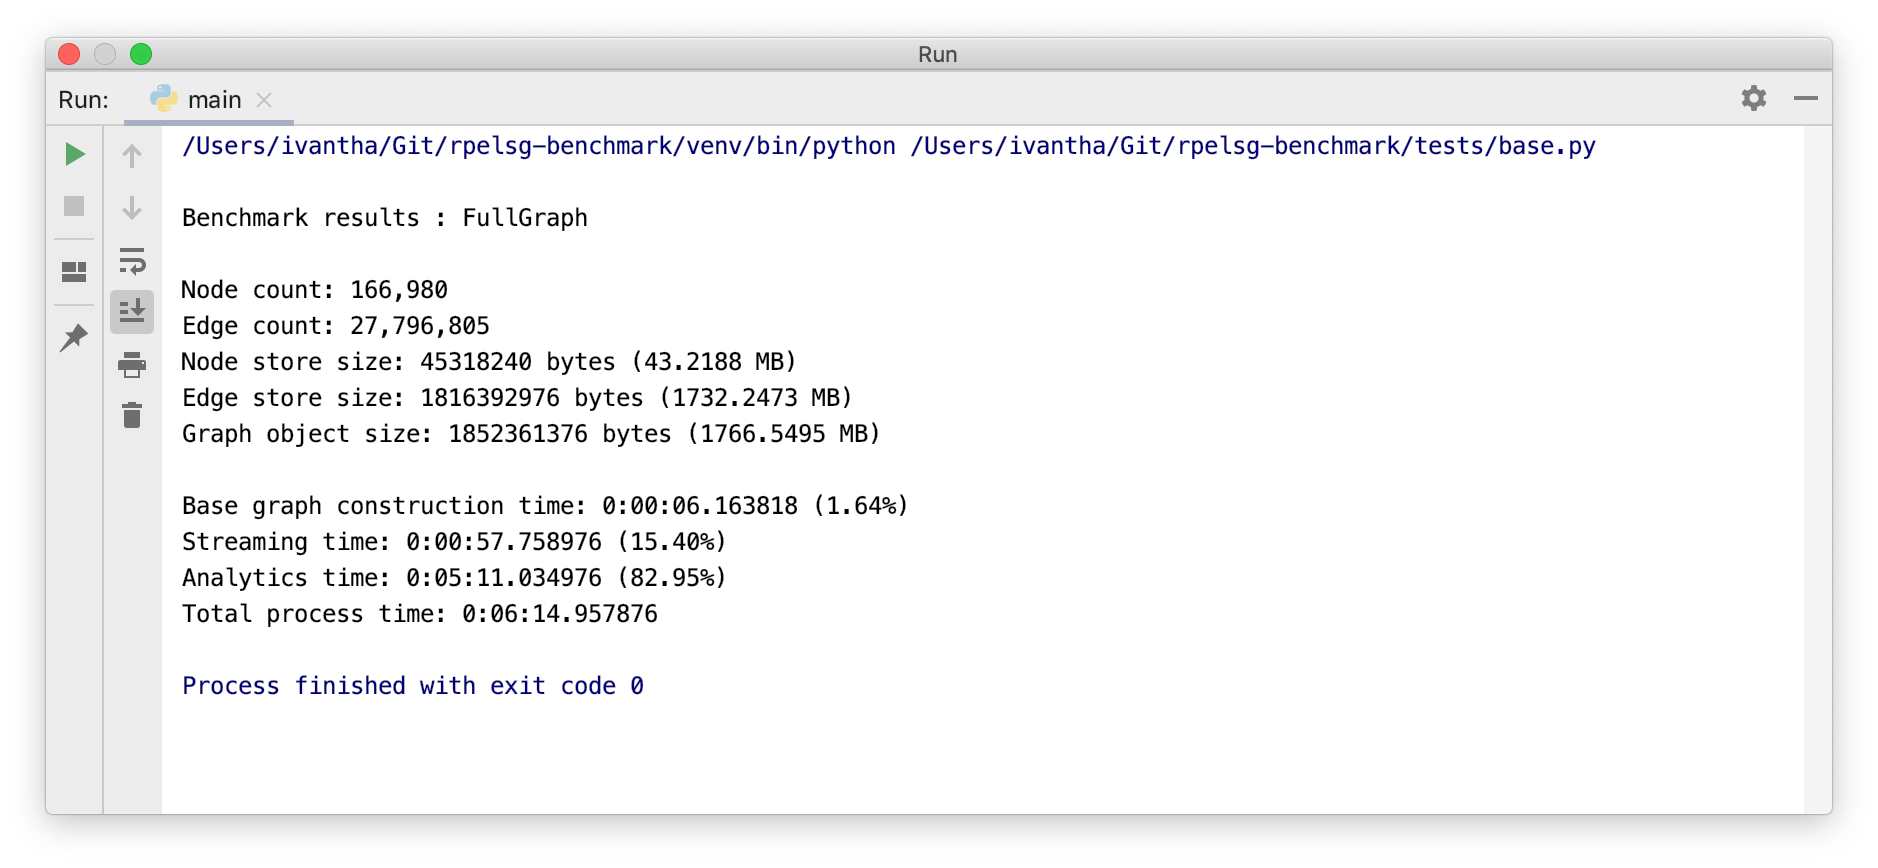
\includegraphics[width=0.8\textwidth]{images/fgraph-results}
    \caption{Full graph results}
\end{figure}

\begin{figure}[H]
    \centering
    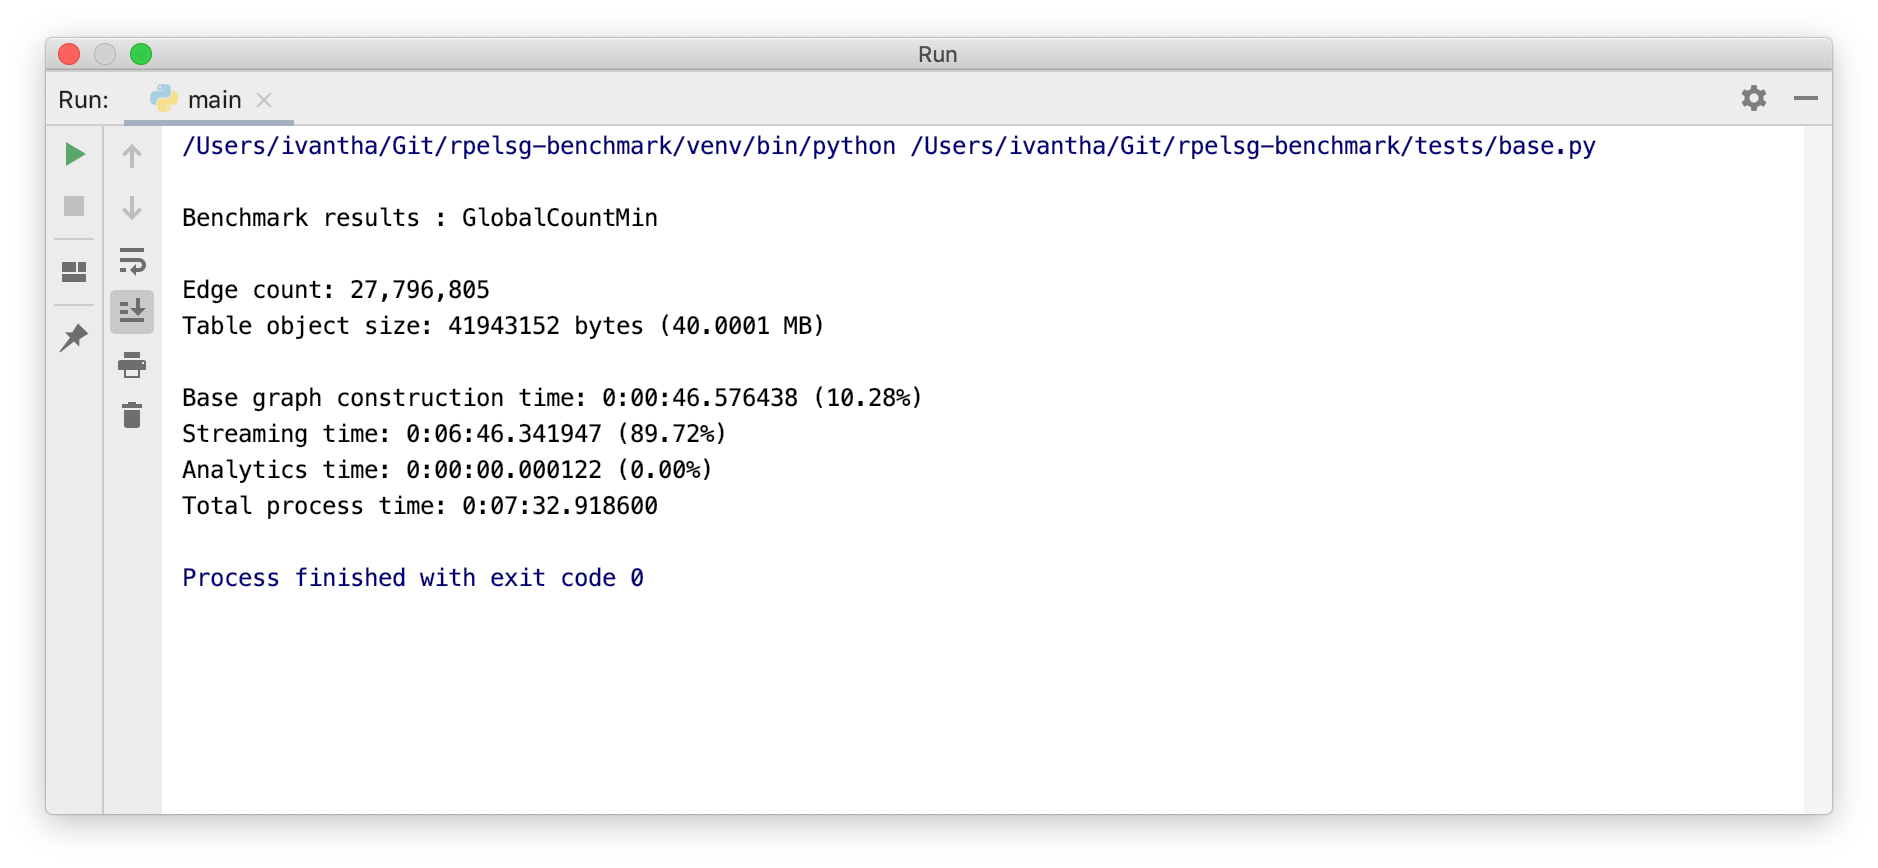
\includegraphics[width=0.8\textwidth]{images/gcm-results}
    \caption{Global CountMin results}
\end{figure}

\begin{figure}[H]
    \centering
    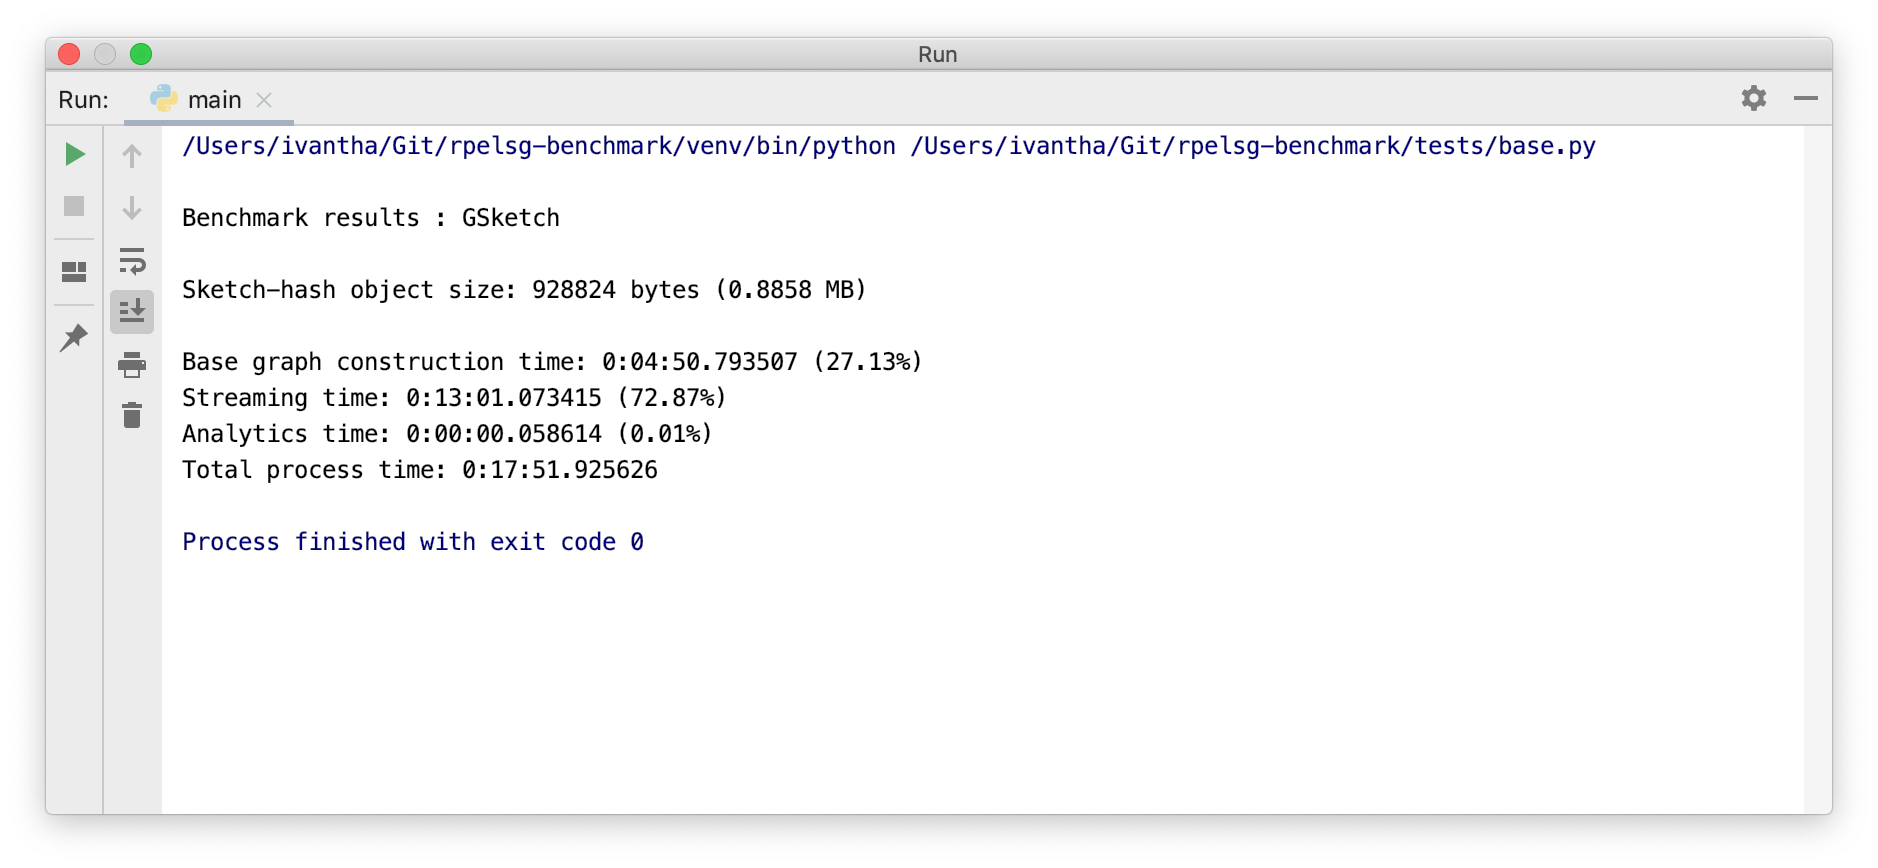
\includegraphics[width=0.8\textwidth]{images/gsketch-results}
    \caption{gSketch results}
\end{figure}

\begin{figure}[H]
    \centering
    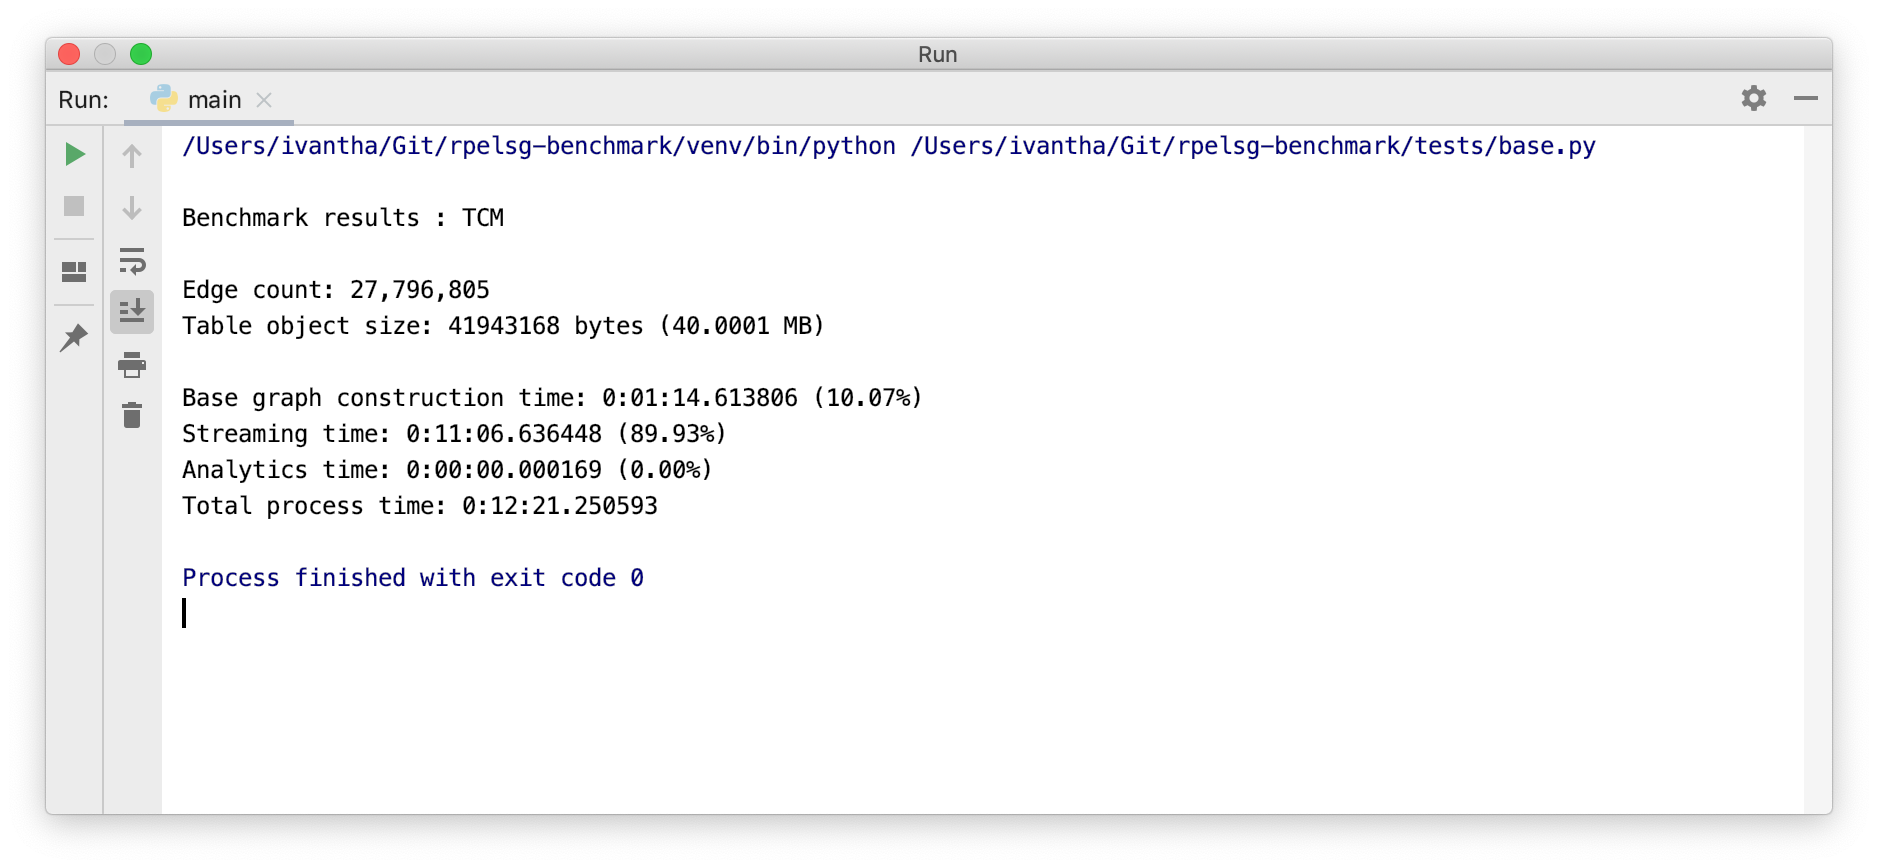
\includegraphics[width=0.8\textwidth]{images/tcm-results}
    \caption{TCM results}
\end{figure}

\newpage
\chapter{Evaluation Plan} \label{evplan}

\section{Environment}

\paragraph{}
All the experiments will be done in an EC2 instance on Amazon Web Services (AWS). The instance will optimally have 4 virtual CPU cores, 32 GB memory and running Ubuntu 16.04. All the algorithms including the proposed sketch will be implemented using Python. 

\section{Datasets}

\paragraph{}
4 datasets have been chosen to evaluate the performance of the proposed sketching technique. Three of the datasets are real world graphs while the fourth dataset will be generated randomly. Details of these datasets are as below. 

\subsection{unicorn-wget-dataset}

\begin{itemize}
    \item \textbf{URL} - \url{https://dataverse.harvard.edu/dataverse/unicorn-wget}
    \item \textbf{Description} - A dataset containing source and target IP addresses of computers in a simulated attack network.
    \item \textbf{Node count} - 166,980
    \item \textbf{Edge count} - 27,796,805
\end{itemize}

\subsection{web-NotreDame}

\begin{itemize}
    \item \textbf{URL} - \url{https://snap.stanford.edu/data/web-NotreDame.html}
    \item \textbf{Description} - Nodes represent pages from University of Notre Dame (domain nd.edu) and directed edges represent hyperlinks between them.
    \item \textbf{Node count} - 325,729
    \item \textbf{Edge count} - 1,497,134
\end{itemize}

\subsection{email-EuAll}

\begin{itemize}
    \item \textbf{URL} - \url{https://snap.stanford.edu/data/email-EuAll.html}
    \item \textbf{Description} - The network was generated using email data from a large European research institution for a period from October 2003 to May 2005 (18 months).
    \item \textbf{Node count} - 265,214
    \item \textbf{Edge count} - 420,045
\end{itemize}

\subsection{Randomly generated dataset}

\begin{itemize}
    \item \textbf{Description} - A randomly generated graph.
    \item \textbf{Node count} - 500,000
    \item \textbf{Edge count} - 100,000,000
\end{itemize}

\section{Metrics} \label{metrics}

\paragraph{}
Following metrics will be used to measure the performance of sketching algorithms. 

\subsection{Average relative error}

\paragraph{}
Relative error is defined as,

\begin{equation}
    er(Q) =  \frac{\tilde{f}'(Q) - f(Q)}{f(Q)} = \frac{\tilde{f}'(Q)}{f(Q)} -1 
\end{equation}

\paragraph{}
Given a set of m queries, $\{ Q_1 , ....., Q_m \}$, average relative error is defined by averaging the relative errors over all queries $Q_i$ for \(i \in [1,m]\) as,

\begin{equation}
    e(Q) =  \frac{\sum_{i=1}^{k} er(Q_i)}{m}
\end{equation}

\subsection{Number of effective queries}

\paragraph{}
A query is said to be effective if the error, $\tilde{f}'(Q) - f(Q), < G_0$,  where $G_0$ is a predefined value.

\begin{equation}
    g(Q) =  \frac{\left | \{\,q\, |   \left |\tilde{f}'(q) - f(q)\right | \leq G_0, \,q \, \epsilon  \,Q\} \, \right|}{|Q|}*100
\end{equation}

\section{Experiments}

\paragraph{}
Five types of experiments will be performed on all the datasets for all the implemented sketching algorithms. 

\subsection{Edge queries}

\begin{enumerate}
    \item Heavy edges - Studying the performance when estimating heavy edges
    \item Compare with gSketch
    \item Compare with TCM
    \item Compare with GSS
    \item Same space for a set of problems
\end{enumerate}

\subsection{Node queries}

\begin{enumerate}
    \item Heavy nodes - Studying the performance when estimating heavy nodes
    \item Conditional heavy hitters - Studying the performance when finding the most popular neighbors to the most popular nodes 
\end{enumerate}

\subsection{Path queries}

\begin{enumerate}
    \item Reachability queries - Studying the performance when finding the reachability between two nodes
\end{enumerate}

\subsection{Graph analytics}

\begin{enumerate}
    \item Subgraph queries - Studying the performance when estimating subgraph queries
    \item Heavy triangle connections 
\end{enumerate}

\subsection{Efficiency}

\paragraph{}
Measuring the efficiency of the proposed sketch with respect to the metrics given in section \ref{metrics} while changing, 

\begin{itemize}
    \item Number of hash functions
    \item Allocated memory 
\end{itemize}

\newpage
\chapter{Research Tools}

\paragraph{}
This section introduces the tools used throughout the research so far. 

\section{Reference Managing Software}

\subsection{Mendeley}

\paragraph{}
Mendeley was our initial choice for reference management. However the 1 GB cloud sync limit posed a big problem as there were lot of reference material to be saved. Despite the reputation of Mendeley, we identified some bugs in the software when it started updating. 

\subsection{Zotero}

\paragraph{}
We switched to Zotero in order to eliminate the disadvantages of Mendeley. Zotero has a rich set of features to manage a local hard copy of the articles. The software allows users to store either a soft link to the file or a hard copy. So this allowed us to keep a backup of the Zotero library and sync the folder to our cloud storage which had much more capacity. Also there was a plugin called \emph{ZotFile} which facilitated us to name the stored files according to our desired collections. 

\section{Document Typesetting}

\subsection{LaTeX}

\paragraph{}
LaTeX was used in compiling this report. There was no decision to be made regarding this as LaTeX is the de facto standard of academic documents. 

\section{Publication Platforms}

\begin{itemize}
    \item ResearchGate
    \item arXiv
\end{itemize}

\section{Version Controlling}

\subsection{Git}

\paragraph{}
Version Controlling was used with both the algorithm implementation and the documents that were drafted in LaTeX. This made it easy to switch to previous points in time and work in branches. 

\newpage
\chapter{Improvements based on the last feedback}

\begin{itemize}
    \item Research title was formatted so that every word start from a capital letter. 
    \item Academic year and subject was added to the cover page. 
    \item Numbering of the pre-content section was formatted to roman numerals. 
    \item Avoided headings such as 1.0 etc. 
    \item Formatting was fixed in \emph{List of Figures} to add the prefix of \emph{Figure} to every entry. 
    \item Motivation was added as another paragraph in the introduction. 
    \item All the included figures and tables were referred within the content. 
    \item Weak research question was improved. 
    \item Research methodology was completly rewritten including a diagram of the research design. 
    \item IEEE reference style was used throughout the whole report. 
\end{itemize}

% \addcontentsline{toc}{section}{References}
\bibliographystyle{unsrt}
\bibliography{cat}

\end{document}